 \documentclass[final,3p,times,11pt,onecolumn]{myElsarticle}
\usepackage{float}
\usepackage{times}
\usepackage[utf8]{inputenc}
\usepackage[english]{babel}
\usepackage[T1]{fontenc}
\usepackage{geometry}
\usepackage{color}
\usepackage{soul}
\usepackage{cancel}
\usepackage{subfigure}
\usepackage{enumerate}
\usepackage{amsmath,amsthm,amsfonts,amssymb}
\usepackage{amsthm}
\usepackage{multirow}
\usepackage{graphicx}
\graphicspath{{./figs/}}
\numberwithin{equation}{section}
\usepackage{spverbatim}
\usepackage{fancyhdr}
\usepackage{listings} 
\usepackage{lineno}
\usepackage[none]{hyphenat}
\date{\today}
\setcounter{secnumdepth}{3}
\providecommand{\abs}[1]{\lvert#1\rvert}
\providecommand{\norm}[1]{\lVert#1\rVert}
\setlength\parindent{12pt}		

%\linenumbers

\newcommand{\COM}[1]{{\color{green} #1}}
\newcommand{\HA}[1]{{\color{red} #1}}
\newcommand{\CIP}[1]{{\color{blue} #1}}
\newcommand{\CMV}[1]{{\color{orange} #1}}


\begin{document}

\begin{frontmatter}

\title{A pressure-velocity coupling strategy based on SIMPLEC: the COMPLEX algorithm}
%% A second-neighbor extended correction for segregated p-v coupling algorithms
 
\author[a]{Horacio J. Aguerre}
\author[b,a]{Cesar I. Pairetti}
\author[a,b]{Cesar M. Venier}
\author[a,c]{Santiago Marquez Damian}
\author[a,d]{Norberto M. Nigro}

\address[a]{Centro de Investigación de Métodos Computacionales, CONICET-UNL, Santa Fe, Argentina}
\address[b]{Escuela de Ingenier\'ia Mec\'anica, Facultad de Ciencias Exactas, Ingenieria y Agrimensura, Universidad Nacional de Rosario, Rosario, Argentina}
\address[c]{Facultad Regional Santa Fe, Universidad Tecnologica Nacional, Santa Fe, Argentina}
\address[d]{Facultad de Ingeniería y Ciencias Hídricas, Universidad Nacional del Litoral, Santa Fe, Argentina}

%Start of abstract
\begin{abstract}
This paper introduces the COMPLEX algorithm which is an enhancement of  SIMPLEC . The new approach is based on considering the neighbour velocity approximation of SIMPLEC as a Taylor expansion. Using this assumption, a first-order term is included in the neighbour approximation leading to a second-order estimate. The new term includes a velocity gradient which is assumed to be a scalar matrix  where its scalar value is defined by solving a mass balance equation. The stability of the method is analysed with a Fourier decomposition of the error showing significant benefits in the convergence rate when comparing it with SIMPLE and SIMPLEC. In the same line, the new method is tested in two typical laminar flow problems where COMPLEX exhibits better convergence properties in the range of high relaxation factors and showing similar performances in for the remaining conditions.
\end{abstract}

\begin{keyword}
Segregated algorithms \sep Segregated method \sep Collocated grids \sep Finite Volume Method 
\end{keyword}
\end{frontmatter}

%%%%%%%%%%%%%%%%%%%%%%%%%%%%%%%%%%%%%
\section{Introduction}

{\color{red}Owing to the low computational efficiency and large memory require-
ment, it has not been widely applied in engineering problems such as
built-environment; however, it is currently successfully used in aero-
space and multiphase flow simulation. Coupled methods have been
widely employed for the computation of compressible flows, whereas
segregated methods have been preferred for the computation of in-
compressible flows. Unlike a coupled solution, a segregated method
solves velocity and pressure fields separately or consecutively. It ex-
hibits the advantages of reduced computer memory and CPU time re-
quirements [13], rendering it computationally more efficient [14] for
analyzing incompressible fluid [15], which is the case in built-en-
vironment simulation.}

\begin{enumerate}
    \item {\color{red} Introducción a CFD en FVM, metodos de acoplamiento p-v: Monolitico vs Segregados. Relevancia de los metodos segregados.} 
    \item {\color{red} Establecer problemática de los segregados: costo computacional de iterar. Variantes respecto a SIMPLE y objetivos de cada variante: SIMPLE con relajación de P, SIMPLEC mejora sobre SIMPLE, PISO mejora sobre SIMPLE}
    \item {\color{red} Introduccion a COMPLEX, que motivo esta propuesta, en que se basa, problematica que viene a solucionar}
    \item {\color{red} Descripcion de las secciones del paper.}
\end{enumerate}

\begin{enumerate}
\item In the context of Computational Fluid Dynamics (CFD) based on the Finite Volume Method (FVM), pressure-velocity coupling
within Navier-Stokes equations may be solved through several strategies. Broadly, the methods may be classified as direct (monolithic)
or segregated. The first one consists on solving one system of equations which includes all the governing equations at once for all the unknowns. Examples of this approach may be found in the literature {\color{red} CITAS Mazhar x2, Chen, Darwish x2, Uoric(Jasak)}. In these works the pressure and velocity are assembled together in a unique system of equations where the non-linearity of the convective term is treated iteratively. Segregated algorithms, in contrast, solves separately for a unique variable at a time. The procedure is iterative and ends when the unknowns satisfy a convergence criteria. Within these group of methods, the penalty method \cite{temam1968methode}, the artificial compression method \cite{harten1977artificial} and pressure correction and projection strategies are among the most adopted {\color{red} CHORIN}.
In the pressure correction/projection methods, an initial estimation of the velocity is corrected by means of a pressure equation where the velocity field is forced to satisfy the divergence free condition. FS MAC y caemos en simple y posteriormente en su familia.



%split the full-coupled system in several sub-systems;
each of them aiming to provide an estimation of a particular field.



%In these methodologies, the variables of the problem can be stored in the same or different spatial locations, which gives place to grid arrangements known as collocated or staggered respectively. The staggered grids have the advantage of avoiding interpolations and thus prevents the appearance of spurious oscillations on the unknown fields. On the other hand, collocated grid arrangements re more suitable for unstructured meshes which are mandatory to address practical applications involving complex geometries.


\item In 1972, Spalding and Patankar [12] proposed the SIMPLE algorithm for heat, mass and momentum transfer. With the SIMPLE
algorithm, pressure and velocity are decoupled so as to be solved sequentially. 

%There are two main assumptions in SIMPLE algorithm:

%\begin{itemize}
%\item The initial pressure and velocity are given independently
%\item The velocity corrections at the neighbours are negligible. 
%\end{itemize}

%These two approximations slow down the convergence to a coupled system.
In terms of overcoming the first assumption, Patankar [10, 11]
proposed the SIMPLER algorithm. This improvement consists on solving an initial pressure equation based on the previous velocity
values.
Further enhancements have been proposed to overcome the second assumption. In 1984, Raithby and van Doormal [14]
SIMPLEC algorithm which propose a simple approximation for the velocity correction in the neighbours cells. In 1986, Issa [2]
presented an operator-splitting scheme for implicitly discretized equations called PISO algorithm. Thus, the neighbors’ contribution
to the velocity correction is under consideration. Tao et al. [? ? ] improved the SIMPLER algorithm developing a fully implicit
alternative named CLEAR without using the pressure correction equation. The CLEAR algorithm discards the second assumption
so that the convergence rate is dramatically increased. However, an unexpected oscillation in the calculation procedure deteriorates
the robustness. To overcome this issue, they developed the IDEAL [? ] algorithm which improves robustness applying several
corrector steps. More recently, improvements have focused on stability for problems with high Reynolds number solved on fine
meshes [? ? ]. A better understanding on the differences between SIMPLE-family algorithms has been accomplished by means of
Fourier analysis [5, 6, 7, 8, 9].
Despite the aforementioned efforts to improve SIMPLE assumptions, there are still possibilities to enhance performance and
robustness of the algorithms.

\item In this work, an extension of the SIMPLEC correction is proposed, based on applying a second order
Taylor approximation to estimate velocity correction values on neighbour cells. The construction of this approximations and its
usage within the algorithm require further assumptions, discussed in detail on the next sections.

\item This article is organized as follows: section 2 describes the SIMPLE and SIMPLEC algorithms, which are the starting point
to define COMPLEX, in section 3, by the assumptions employed to obtain the new approximation of neighbour correction terms.
A stability analysis, based on Fourier decomposition, between the three algorithms is presented in section 4. Then, the results of
each algorithm for two well-known benchmark cases, solved on two flow regimes using three mesh-size on each, are compared in section 5. The conclusions on section 6 summarizes the advantages and limitations of the proposed method, discussing further
improvements that could be applied in the future.
\end{enumerate}




\section{Theoretical background} \label{sec:theory}
This section starts with a description of the SIMPLE algorithm which is followed by the foundations of the SIMPLEC method. After this basis, the method proposed in this work is formally presented.

The continuum incompressible Navier-Stokes equations may be presented as:

\begin{align}
\displaystyle \frac{\partial \boldsymbol{u}}{\partial t} + \nabla \cdotp (\boldsymbol{u} \boldsymbol{u}) &= -\nabla p + \nu\, \Delta \boldsymbol{u} + \boldsymbol{\Phi},
\label{eq:mom1}
\\
\displaystyle \nabla \cdotp \boldsymbol{u} &= 0, 
\label{eq:mass1}
\end{align}

\noindent where $\displaystyle p = (\mathcal{P}/\rho)$, $\rho$ is the mass density, $\mathcal{P}$ is the pressure field, $\boldsymbol{u} = (u,v,w)$ is the velocity field, $\nu$ is the kinematic viscosity and $\mathbf{\Phi}$ is a momentum source term.
Based on the FVM \cite{jasak}, the Eqs.~(\ref{eq:mass1}) and~(\ref{eq:mom1}) may be discretized as:

\begin{align}
a_P\,\boldsymbol{u}_P + \sum_{N} a_{N}\,\boldsymbol{u}_{N} &= b_P\, \boldsymbol{u}^0_P + \boldsymbol{\Phi}_P - \nabla p_P,
\label{eq:umom1}
\\
\sum_{f} \boldsymbol{u}_{f} \cdotp \textbf{S}_{f} &= 0, 
\label{eq:mass2} 
\end{align}
where the subscript $P$ indicates the cell values, $N$ indicates neighbour cell values and $f$ refers to face values, $b_P\, \boldsymbol{u}^0_P$ is the contribution of the previous time-step or iteration. The value of $b_P$ is function of the temporal scheme in transient solvers and of the relaxation factor in steady-state solvers, $\textbf{S}_{f}$ is the face-normal vector,  $a_P$ and $a_{N}$ are the diagonal and off-diagonal momentum matrix coefficients respectively and the gradient $\nabla p_P$ is computed by linear interpolation of first neighbours values of that field.

An alternative to solve the system of Eqs.~(\ref{eq:umom1}) and (\ref{eq:mass2}) is to isolate the velocity $\mathbf{u}_{P}$ from Eq.~(\ref{eq:umom1}) and introduce it in Eq.~(\ref{eq:mass2}). Then,
\begin{equation}
\label{Eq:UpIsolated}
\boldsymbol{u}_P
=
\dfrac
{
-\sum_{N} a_{N}\,\boldsymbol{u}_{N}
+
b_P\, \boldsymbol{u}^0_P 
+ 
\boldsymbol{\Phi}_P 
- 
\nabla p_P}
{a_P}.
\end{equation}
To simplify the notation, the variable $\boldsymbol{H}$ is defined,
\begin{equation}
\boldsymbol{H}
\equiv
-\sum_{N} a_{N}\,\boldsymbol{u}_{N}
+
b_P\, \boldsymbol{u}^0_P 
+ 
\boldsymbol{\Phi}_P
\end{equation}
Consequently, the Eq.~(\ref{Eq:UpIsolated}) may be expressed as,
\begin{equation}
\label{Eq:UpIsolatedH}
\boldsymbol{u}_P
=
\dfrac
{
\boldsymbol{H}
- 
\nabla p_P}
{a_P}.
\end{equation}
After this, last equation is replaced in Eq.~(\ref{eq:mass2}),
\begin{equation}
\sum_{f} 
\left(
\boldsymbol{u}_{P} 
\right)_f
\cdotp 
\textbf{S}_{f} 
=
\sum_{f} 
\left(
\dfrac
{
\boldsymbol{H}
- 
\nabla p_P}
{a_P}
\right)_f
\cdotp 
\textbf{S}_{f}
= 
0,
\end{equation}
where the operator $(\cdot)_f$ interpolates linearly cell values into faces. Finally, a expression for the pressure is obtained,
\begin{equation}
\label{Eq:firstPressureEq}
\sum_{f} 
\left(
\dfrac
{
\nabla p_P}
{a_P}
\right)_f
\cdotp 
\textbf{S}_{f}
=
\sum_{f} 
\left(
\dfrac
{
\boldsymbol{H}
}
{a_P}
\right)_f
\cdotp 
\textbf{S}_{f}.
\end{equation}
At this point the discretized Navier-Stokes equations is represented by two linear system of equations, one for the velocity, Eq.~(\ref{Eq:UpIsolatedH}) and the other one for the pressure, Eq.~(\ref{Eq:firstPressureEq}).

\subsection{The SIMPLE algorithm on collocated grids}

In the SIMPLE algorithm, a subdivision of the velocity is proposed. With this in mind, the velocity and pressure fields may be considered as the contribution of two parts,
\begin{align}
\label{Eq:velocitySubdiv}
\boldsymbol{u}_P
= 
\boldsymbol{u}_P^{*} 
+
\boldsymbol{u}_P^{'}
\\
\label{Eq:pressureSubdiv}
p_P
=
p_P^{*} 
+
p_P^{'}
\end{align}
where $\boldsymbol{u}_P^{*}$, $p_P^{*}$ are the velocity and pressure predictions, and $\boldsymbol{u}_P^{'}$, $p_P^{*}$ are corrections fields. In particular, the subdivision of the velocity leads to an analogous separation of the variable $\boldsymbol{H}$,
\begin{equation}
\label{Eq:HSubDivision}
\boldsymbol{H} 
=
\boldsymbol{H}^{*}
+
\boldsymbol{H}^{'},
\end{equation}
where,
\begin{align}
\label{Eq:HStar}
\boldsymbol{H}^{*} 
&\equiv -\sum_{N} a_{N}\,\boldsymbol{u}_{N}^{*}
+
b_P\, \boldsymbol{u}^0_P 
+ 
\boldsymbol{\Phi}_P,
\\
\label{Eq:HPrima}
\boldsymbol{H}^{'}
&\equiv -\sum_{N} a_{N}\,\boldsymbol{u}_{N}^{'}. 
\end{align}
Considering these last expressions, the algorithm starts by computing the momentum balance to predict the velocity $\boldsymbol{u}_P^{*}$ using a pressure prediction equal to previous iteration value $p^{*}=p^{0}$,
\begin{equation}
\label{Eq:MomentumPredictor}
\boldsymbol{u}_P^{*}
=
\dfrac
{
\boldsymbol{H}^*
- 
\nabla p_P^{*}}
{a_P}.
\end{equation}
After this, the pressure is computed by introducing the Eq.~(\ref{Eq:HSubDivision}) in the mass balance of Eq.~(\ref{Eq:firstPressureEq}),
\begin{equation}
\label{Eq:pressureEqSubdiv}
\sum_{f} 
\left(
\dfrac
{
\nabla p_P}
{a_P}
\right)_f
\cdotp 
\textbf{S}_{f}
=
\sum_{f} 
\left(
\dfrac
{
\boldsymbol{H}^{*}
+
\boldsymbol{H}^{'}
}
{a_P}
\right)_f
\cdotp 
\textbf{S}_{f}.
\end{equation}
Since the correction velocity values $\boldsymbol{u}_N^{'}$  are not yet computed, an approximation of $\boldsymbol{H}^{'}$ must be proposed. In this sense, the SIMPLE method proposes to neglect the influence of the neighbour velocity correction which is equivalent to neglect,
\begin{equation}
\label{Eq:simpleAproximation}
\boldsymbol{H}^{'} = 0,
\end{equation}
thus, introducing~Eq.~(\ref{Eq:simpleAproximation}) into (\ref{Eq:pressureEqSubdiv}),
\begin{equation}
\sum_{f} 
\left(
\dfrac
{
\nabla p_P}
{a_P}
\right)_f
\cdotp 
\textbf{S}_{f}
=
\sum_f 
\left(
\dfrac
{
\boldsymbol{H}^*
}
{
a_P
}
\right)_f
\cdot
\boldsymbol{S}_f,
\label{eq:div-free5}  
\end{equation}
which determines a Poisson problem for the pressure. Nevertheless, solving this system in a straightforward manner may lead to high-frequency oscillations. The Rhie-Chow correction \cite{rhiechow} reduces this effect in collocated grids, 

\begin{equation}
\label{eq:pEqnSIMPLE2}
\sum_{f} 
\left(
\dfrac
{
\nabla p_P}
{a_P}
\right)_f
\cdotp 
\textbf{S}_{f} 
=
\sum_f 
\left(
\dfrac{
\boldsymbol{H}^*
}
{
a_P
}
\right)_f
\cdot
\boldsymbol{S}_f 
+
\sum_f  
\left[
\left(
\frac{\nabla p_P}{a_P}
\right)_f
- 
\left(
\frac{1}{a_P}
\right)_f 
\nabla p_f
\right]
\cdot 
\boldsymbol{S}_f.
\end{equation}
Reordering Eq.~(\ref{eq:pEqnSIMPLE2}), the pressure equation may be written as,
\begin{equation}\label{eq:pEqnSIMPLE3}
\sum_f \left(\frac{1}{a_P}\right)_f \nabla p_f 
\cdot
\boldsymbol{S}_f 
=  \sum_f \left(\frac{\boldsymbol{H}^*}{a_P}\right)_f \cdot \boldsymbol{S}_f.
\end{equation}
Finally, the velocity value is computing by Eq.~(\ref{Eq:UpIsolatedH}) where the variable $\boldsymbol{H}$ is approximated by $\boldsymbol{H}^{*}$ similarly as done in the mass balance equation,
\begin{equation}
\label{eq:SIMPLECorr}
\boldsymbol{u}_P
=
\dfrac
{
\boldsymbol{H}^*
- 
\nabla p_P}
{a_P}.
\end{equation}
Note that last equation is explicit since the terms r.h.s of last equation are known. The algorithm continues with Eq.~(\ref{Eq:MomentumPredictor}) where the last values of $\boldsymbol{u}_p$ and $p_p$ are considered as $\boldsymbol{u}_p^0$ and $p_p^0$.



% In order to do so, the velocity field $\boldsymbol{u}_P$, originally on cell-centers, needs to be interpolated to the faces obtaining: 
%
% \begin{equation}
% \begin{split}
% \sum_{f} \left( \boldsymbol{H}_P - \frac{1}{a_P} \nabla p_P  \right)_f \cdotp \textbf{S}_{f} = 0 
% \end{split}
% \label{eq:pEq1} 
% \end{equation}
%
%Therefore, the Corrector step may be summarized as:
%
%\begin{enumerate}
%
%\item Assemble and solve the pressure based on Eq.~(\ref{eq:pEq1}):
%
%\begin{equation}
%\begin{split}
%\sum_{f} \left( \frac{1}{a_P} \nabla p'_P \right)_f \cdotp \textbf{S}_{f} = \sum_{f} \boldsymbol{u}^*_f \cdotp \textbf{S}_{f}
%\end{split}
%\label{eq:pEq2} 
%\end{equation}


%\CIP{Si conservamos la forma relativa, aquí habría que meter la explicación de Rhie Chow}

%\item {\color{red}Compute} the face fluxes by adding the new pressure contribution:
%
%\begin{equation}
%\begin{split}
%F_f = \boldsymbol{u}^*_f \cdotp \textbf{S}_{f} -  \left( \frac{1}{a_P}\right)_f \nabla p'_f  \cdotp \textbf{S}_{f}
%\end{split}
%\label{eq:Fhat} 
%\end{equation}
%
%\item Correct the cell-centered velocity field based on the new pressure field, using Eq. (\ref{eq:umom3b})
%
%\begin{equation}\label{eq:umom3b}
%\begin{split}
%\boldsymbol{u}_P = \boldsymbol{u}^*_P - \frac{1}{a_P} \nabla p'_P 
%\end{split}
%\end{equation}
%
%\end{enumerate}

%\fi
%Most of the SIMPLE-family algorithms preserve this general structure. In particular, the SIMPLE algorithm \cite{patankar1972}, originally conceived as a steady state flow solver, adds under-relaxation factors to obtain a stable solution. Another variant is the PISO {\color{red}(Pressure-Implicit with Splitting of Operators)} algorithm, which relies on iterating the Corrector step a given number of times to ensure a correct coupling between pressure and velocity for transient flow problems \cite{issa,issa2}. {\color{red} The SIMPLE-PISO combined technique has been largely adopted in several computational codes (e.g. OpenFOAM(R) \cite{ofpg}) to address transient incompressible flow problems due to its beneficial convergence features. It consists on iterating the corrector steps until a certain mass conservation criteria is fulfilled (as in PISO) and iterating the whole sequence (Momentum Predictor and Corrector Step) several times until both mass and momentum equations are verified for each time step. This algorithm will be adopted in the present work.}

\subsection{Improving the neighbor approximation: the SIMPLEC algorithm}
The SIMPLEC~\cite{vanDoormal} algorithm proposes an aproximation of the neighbour velocity correction $\boldsymbol{u}_N'$,
\begin{equation}
\label{Eq:simplecAproximation}
\boldsymbol{u}_N'
=
\boldsymbol{u}_P'
\end{equation}
and therefore the Eq.~(\ref{Eq:HPrima}) may be expressed as,
\begin{equation}
\label{eq:H_SIMPLEC}
\boldsymbol{H}'= \left(-\sum_N a_N\right) \boldsymbol{u}'_P.
\end{equation}
To include last expression in Eq.~(\ref{Eq:pressureEqSubdiv}), it must be expressed as function of the  pressure. For this, a expression for $\boldsymbol{u}^{'}$ is derived by subtracting Eq.~(\ref{Eq:MomentumPredictor}) from Eq.~(\ref{Eq:UpIsolated}),
\begin{equation}
\label{Eq:UPrimaIsolated}
\boldsymbol{u}_P'
=
\dfrac
{
\boldsymbol{H}'
- 
\left(
\nabla p_P
-
\nabla p_P^{0}
\right)
}
{a_P},
\end{equation}
which in combination with Eq.~(\ref{eq:H_SIMPLEC}) determines an expression of $\boldsymbol{H}'$ as function of the pressure,
\begin{equation}
\label{Eq:HPrima}
\boldsymbol{H}'
= 
\dfrac
{
\left(
\tilde{a}_P
-
a_P
\right)
}
{
\tilde{a}_P
}
\left(
\nabla p_P
-
\nabla p_P^{0}
\right).
\end{equation}
being $\tilde{a}_P$ a definition given by,
\begin{equation}
\tilde{a}_P
\equiv
a_P + \sum_{N} a_{N}.
\end{equation}
Subsequently, introducing Eq.~(\ref{Eq:HPrima}) in Eq.~(\ref{Eq:pressureEqSubdiv})

\begin{equation}
\label{Eq:pressureReplacedSimplec}
\sum_{f} 
\left(
\dfrac
{
\nabla p_P}
{a_P}
\right)_f
\cdotp 
\boldsymbol{S}_{f}
=
\sum_{f} 
\left(
\dfrac
{
\boldsymbol{H}^{*}
}
{a_P}
\right)_f
\cdotp 
\boldsymbol{S}_{f}
+
\sum_f
\left[
\dfrac
{
\left(
\tilde{a}_P
-
a_P
\right)
}
{
\tilde{a}_P\,a_P
}
\left(
\nabla p_P
-
\nabla p_P^{0}
\right)
\right]_f
\cdot
\boldsymbol{S}_{f},
\end{equation}
and simplifying and reordering,
\begin{equation}
\label{Eq:pressureReplacedSimplec2}
\sum_{f} 
\left(
\dfrac
{
\nabla p_P}
{\tilde{a}_P}
\right)_f
\cdotp 
\boldsymbol{S}_{f}
=
\sum_{f} 
\left(
\dfrac
{
\boldsymbol{H}^{*}
}
{a_P}
\right)_f
\cdotp 
\boldsymbol{S}_{f}
+
\sum_f
\left[
\left(
\dfrac{1}
{\tilde{a}_P}
-
\dfrac{1}
{a_P}
\right)
\nabla p^{0}
\right]_f
\cdot
\boldsymbol{S}_f.
\end{equation}
The pressure equation is obtained by including an analogous Rhie-Chow correction:

\begin{equation}
\label{eq:pEqnSIMPLEC2}
\begin{array}{ccc}
&
\sum_{f} 
\left(
\dfrac
{
\nabla p_P}
{\tilde{a}_P}
\right)_f
\cdotp 
\boldsymbol{S}_{f} 
=
\sum_{f} 
\left(
\dfrac
{
\boldsymbol{H}^{*}
}
{a_P}
\right)_f
\cdotp 
\boldsymbol{S}_{f}
+
\sum_f
\left[
\left(
\dfrac{1}
{\tilde{a}_P}
-
\dfrac{1}
{a_P}
\right)
\nabla p^{0}
\right]_f
\cdot
\boldsymbol{S}_f
&
\\
&+& \\
&
\sum_f
\left\lbrace
\left(
\dfrac
{
\nabla p
}
{\tilde{a}_P}
\right)_f
-
\left(
\dfrac
{1}
{\tilde{a}_P}
\right)_f
\nabla p_f
+
\left(
\dfrac
{1}
{\tilde{a}_P}
-
\dfrac
{1}
{a_P}
\right)_f
\nabla p^{0}_f
-
\left[
\left(
\dfrac
{1}
{\tilde{a}_P}
-
\dfrac
{1}
{a_P}
\right)
\nabla p^0
\right]_f
\right\rbrace
\cdot
\boldsymbol{S}_f,
&
\end{array}
\end{equation}
Then, simplifying,
\begin{equation}
\sum_f
\left[
\left(
\dfrac
{1}
{\tilde{a}_P}
\right)_f
\nabla p_f
\right]
\cdot 
\boldsymbol{S}_f
= 
\sum_f 
\left[
\frac{1}{a_P}
\left(
\boldsymbol{H}^*
\right)
\right]_f 
\cdot
\boldsymbol{S}_f
+
\sum_f
\left[
\left(
\dfrac
{1}
{\tilde{a}_P}
-
\dfrac
{1}
{a_P}
\right)_f
\nabla p^{0}_f
\right]
\cdot
\boldsymbol{S}_f.
\label{eq:pEqnSIMPLEC}
\end{equation}

The velocity is computed by employing the approximation of Eq.~(\ref{Eq:HPrima}) in Eq.~(\ref{Eq:UpIsolatedH}):

\begin{equation}
\label{eq:uCorrSIMPLEC}
\boldsymbol{u}_P 
=
\dfrac
{
\boldsymbol{H}^*
- 
\nabla p_P}
{a_P}
+
\dfrac
{
\left(
\tilde{a}_P
-
a_P
\right)
}
{
\tilde{a}_P\,a_P
}
\left(
\nabla p_P
-
\nabla p_P^{0}
\right).
\end{equation}
and reordering,
\begin{equation}
\label{Eq:velocitySimplec}
\boldsymbol{u}_P 
=
\dfrac
{
\boldsymbol{H}^*
- 
\nabla p_P}
{\tilde{a}_P}
+
\left(
\dfrac{1}
{\tilde{a}_P}
-
\dfrac{1}
{a_P}
\right)
\nabla p^{0}.
\end{equation}


The only difference between SIMPLE and SIMPLEC are the coefficients in the Corrector step. Nevertheless, this slight modification shows a significant improvement in the stability  and convergence properties of the algorithm \cite{liu}. In the spirit of using better approximation for the neighbors correction values, we propose the following method.

\section{Enhancement of SIMPLEC: the COMPLEX method}
\label{sec:COMPLEX}

In order to estimate the value of $\boldsymbol{u}_N'$ in Eq.~(\ref{Eq:HPrima}), a second order Taylor approximation is proposed,
\begin{equation}\label{eq:uNTaylor}
\boldsymbol{u}_N' = \boldsymbol{u}_P' + \boldsymbol{x}_{PN}\cdot 
\nabla \boldsymbol{u}_f'.
\end{equation}

Then, the $\boldsymbol{H}'$ variable may be expressed as,
\begin{equation}
\label{Eq:HPrimaComplex}
\boldsymbol{H}'
=
\left(
-\sum_N a_N
\right)
\boldsymbol{u}_P' 
+
\left(
-\sum_N a_N
\right)
\left(
\boldsymbol{x}_{PN}\cdot 
\nabla \boldsymbol{u}_f'
\right),
\end{equation}
which combined with Eq.~(\ref{Eq:UPrimaIsolated}) reads as follows,
\begin{equation}
\label{Eq:HPrimaComplexReady}
\boldsymbol{H}'
= 
\dfrac
{
\left(
\tilde{a}_P
-
a_P
\right)
}
{
\tilde{a}_P
}
\left(
\nabla p_P
-
\nabla p_P^{0}
\right)
+
\dfrac{a_P}{\tilde{a}_P}
\,
\delta_P,
\end{equation}
where $\delta_P$ is defined as the second term of the r.h.s of Eq.~(\ref{Eq:HPrimaComplex}) which is named in this paper as the complex term,
\begin{equation}
\delta_P 
\equiv 
\left(
-\sum_N a_N
\right)
\left(
\boldsymbol{x}_{PN}\cdot 
\nabla \boldsymbol{u}_f'
\right),
\end{equation}
Including Eq.~(\ref{Eq:HPrimaComplexReady}) in Eq.~(\ref{Eq:pressureEqSubdiv}) and following an analogous derivation as done from Eq.~(\ref{Eq:pressureReplacedSimplec}) up to Eq.~(\ref{eq:pEqnSIMPLEC}), the following pressure equation is obtained for the complex algorithm,
\begin{equation}
\label{Eq:pressureComplex}
\sum_f
\left[
\left(
\dfrac
{1}
{\tilde{a}_P}
\right)_f
\nabla p_f
\right]
\cdot 
\boldsymbol{S}_f
= 
\sum_f 
\left[
\frac{1}{a_P}
\left(
\boldsymbol{H}^*
\right)
\right]_f 
\cdot
\boldsymbol{S}_f
+
\sum_f
\left[
\left(
\dfrac
{1}
{\tilde{a}_P}
-
\dfrac
{1}
{a_P}
\right)_f
\nabla p^{0}_f
\right]
\cdot
\boldsymbol{S}_f
+
\sum_f
\left(
\dfrac{\delta_P}{\tilde{a}_P}
\right)_f
\cdot
\boldsymbol{S}_f.
\end{equation}
The velocity is computed including the approximation of Eq.~(\ref{Eq:HPrimaComplex}) in Eq.~(\ref{Eq:UpIsolatedH}),
\begin{equation}
\label{Eq:velocityComplex}
\boldsymbol{u}_P 
=
\dfrac
{
\boldsymbol{H}^*
- 
\nabla p_P}
{\tilde{a}_P}
+
\left(
\dfrac{1}
{\tilde{a}_P}
-
\dfrac{1}
{a_P}
\right)
\nabla p^{0}
+
\dfrac{\delta_P}
{\tilde{a}_P}.
\end{equation}
The Eqs.~(\ref{Eq:pressureComplex}) and (\ref{Eq:velocityComplex}) are similar to Eqs.~(\ref{eq:pEqnSIMPLEC}) and (\ref{Eq:velocitySimplec}) respectively but for the complex term $\delta_P$ which has as main unknown the face gradient $\nabla \boldsymbol{u}_f'$.

\subsection{Computation of the face gradient}
The face gradient $\nabla \boldsymbol{u}_f' $ is obtained as a linear interpolation of a cell-centred gradient $\nabla \boldsymbol{u}_P'$,
\begin{equation}
\label{Eq:UFaceGradient}
\nabla \boldsymbol{u}_f'
=
(\nabla \boldsymbol{u}_P')_f.
\end{equation}
To obtain an expression for the cell-centred gradient, a derivation starts by including the subdivision of the velocity given in Eq.~(\ref{Eq:velocitySubdiv}) in the mass balance given of Eq.~(\ref{eq:mass2}),
\begin{equation}
\label{Eq:massEqSubdivided}
\sum_{f} 
\left(
\boldsymbol{u}_{P}^*
+ 
\boldsymbol{u}_{P}'
\right)_f
\cdotp \textbf{S}_{f} 
=
\sum_{f} 
\left(
\boldsymbol{u}_{P}^*
\right)_f
\cdotp \textbf{S}_{f}
+
\sum_{f} 
\left(
\boldsymbol{u}_{P}'
\right)_f
\cdotp \textbf{S}_{f}
=
0
\end{equation}
In last equation, the face values $\boldsymbol{u_P}'_f$ are expressed as function of $\nabla \boldsymbol{u}_P'$ by proposing the following first-order Taylor expansion,
\begin{equation}
\label{Eq:TaylorOnFace}
\left(
\boldsymbol{u_P}'
\right)_f
=
\boldsymbol{u_P}'
+
\boldsymbol{x}_{Pf}
\cdot 
\nabla \boldsymbol{u}_P'.
\end{equation} 
Subsequently, this last equation is replaced in  Eq.~(\ref{Eq:massEqSubdivided}),
\begin{align}
\sum_f 
\left(
\boldsymbol{u_P}'
+
\boldsymbol{x}_{Pf}
\cdot 
\nabla \boldsymbol{u}_P'
\right)
\cdot 
\boldsymbol{S}_f 
&=
-\sum_f
\left(
\boldsymbol{u_P}^{*}
\right)_{f} 
\cdot 
\boldsymbol{S}_f
\\
\boldsymbol{u_P}'
\cdot 
\sum_f 
\boldsymbol{S}_f
+
\sum_f 
\left(
\boldsymbol{x}_{Pf}
\cdot 
\nabla \boldsymbol{u}_P'
\right)
\cdot 
\boldsymbol{S}_f
&=
-\sum_f
\left(
\boldsymbol{u_P}^{*}
\right)_{f} 
\cdot 
\boldsymbol{S}_f
\\
\label{Eq:Last}
\sum_f 
\left(
\boldsymbol{x}_{Pf}
\cdot 
\nabla \boldsymbol{u}_P'
\right)
\cdot 
\boldsymbol{S}_f
&=
-\sum_f
\left(
\boldsymbol{u_P}^{*}
\right)_{f} 
\cdot 
\boldsymbol{S}_f
\end{align}
where $\boldsymbol{u_P}^{*}$ is obtained by the momentum predictor, Eq.~(\ref{Eq:MomentumPredictor}),
\begin{equation}
\left(
\boldsymbol{u_P}^{*}
\right)_{f}
=
\left[\frac{1}{a_P}\left(\boldsymbol{H}^* - \nabla p_P^{0}\right)\right]_f.
\end{equation}
Then, a similar form of the Rhie-Chow term given in Eq.~(\ref{eq:pEqnSIMPLE2}) is included,
\begin{equation}
\left(
\boldsymbol{u_P}^{*}
\right)_{f}
=
\left[\frac{1}{a_P}\left(\boldsymbol{H}^* - \nabla p_P^{0}\right)\right]_f
+
\left[
\left(
\frac{\nabla p_P^{0}}{a_P}
\right)_f
- 
\left(
\frac{1}{a_P}
\right)_f 
\nabla p_f^{0} 
\right],
\end{equation}
and simplifying, 
\begin{equation}
\left(
\boldsymbol{u_P}^{*}
\right)_{f}
=
 \left(\frac{\boldsymbol{H}^*}{a_P}\right)_f 
 -
 \left(\frac{1}{a_P}\right)_f \nabla p_f^{0}.
\end{equation}
Replacing in Eq.~(\ref{Eq:Last}),
\begin{equation}
\label{Eq:mainGradEq}
\sum_f 
\left(
\boldsymbol{x}_{Pf}
\cdot 
\nabla \boldsymbol{u}_P'
\right)
\cdot 
\boldsymbol{S}_f
=
-\sum_f
\left[
\left(\frac{\boldsymbol{H}^*}{a_P}\right)_f 
 -
 \left(\frac{1}{a_P}\right)_f \nabla p_f^{0}
 \right]
\cdot 
\boldsymbol{S}_f.
\end{equation}
Last expression allows computing the cell gradient $\nabla \boldsymbol{u}_P'$ as functions of $\boldsymbol{H}^*$ and $\nabla p_f^{0}$ which are known values after the momentum predictor equation is solved. However, the Eq.~(\ref{Eq:mainGradEq}) is underdetermined since the gradient $\nabla \boldsymbol{u}_P'$ requires to define nine unknowns. In order to solve this last underdetermination, an additional approximation is introduced over the gradient definition. In this respect, it is proposed that the gradient $\nabla \boldsymbol{u}_P'$ is a scalar matrix as defined below,
\begin{equation}
\nabla \boldsymbol{u}_P'
=
\alpha_P\,
\boldsymbol{I}
\label{eq:gradApprox}
\end{equation}
Replacing this last definition in Eq.~(\ref{Eq:mainGradEq}),
\begin{align}
\sum_f 
\left(
\boldsymbol{x}_{Pf}
\cdot 
\alpha_P\,
\boldsymbol{I}
\right)
\cdot 
\boldsymbol{S}_f
&=
-\sum_f
\left[
\left(\frac{\boldsymbol{H}^*}{a_P}\right)_f 
 -
 \left(\frac{1}{a_P}\right)_f \nabla p_f^{*}
 \right]
\cdot 
\boldsymbol{S}_f,
\\
\alpha_P
\sum_f 
\left(
\boldsymbol{x}_{Pf}
\cdot 
\boldsymbol{I}
\right)
\cdot 
\boldsymbol{S}_f
&=
-\sum_f
\left[
\left(\frac{\boldsymbol{H}^*}{a_P}\right)_f 
 -
 \left(\frac{1}{a_P}\right)_f \nabla p_f^{*}
 \right]
\cdot 
\boldsymbol{S}_f,
\end{align}
and isolating $\alpha_P$,
\begin{equation}
\alpha_P
=
\dfrac
{-\sum_f
\left[
\left(\frac{\boldsymbol{H}^*}{a_P}\right)_f 
 -
 \left(\frac{1}{a_P}\right)_f \nabla p_f^{*}
 \right]
\cdot 
\boldsymbol{S}_f}
{\sum_f 
\boldsymbol{x}_{Pf}
\cdot 
\boldsymbol{S}_f}
\end{equation}

Finally the face gradient~(\ref{Eq:UFaceGradient}) may be computed using the $\alpha_P$ values interpolated to the faces,
\begin{equation}
\label{Eq:scalarMatrix}
\nabla \boldsymbol{u}_f'
=
\left(
\alpha_P
\right)_f
\boldsymbol{I}.
\end{equation}

\subsection{Relaxation of the complex term}
The COMPLEX method is based on an approximation of the neighbours velocity corrections $\boldsymbol{u}_N'$ as function of a Taylor expansion which is based on the mass balance equation. However, an accurate definition of the gradient for the second term of the Taylor expansion requires additional information which is not available before solving the pressure equation. The unique information obtained with this approach is the trace of the velocity tensor which is opposite to the divergence of the predicted velocity $\boldsymbol{u}^*$. Due to this numerical difficulty, the approximation given in Eq.~(\ref{eq:gradApprox}) is proposed which allows closing the numerical problem at the expense of reducing the whole potential of the original proposal. The use of a scalar matrix as an estimate of the velocity gradient may be interpreted as an isotropic deformation of the velocity correction field $\boldsymbol{u}_P'$. This effect may not be so if this field is recomputed with the new pressure values. Taking this into account, a relaxation of the complex term $\delta_P$ is proposed in order to avoid an excessive estimation of $\boldsymbol{u}_N'$. Introducing a relaxation of the complex term in the Eqs.~(\ref{Eq:pressureComplex}) and (\ref{Eq:velocityComplex}) , 
\begin{equation}
\label{Eq:pressureComplexRelaxed}
\sum_f
\left[
\left(
\dfrac
{1}
{\tilde{a}_P}
\right)_f
\nabla p_f
\right]
\cdot 
\boldsymbol{S}_f
= 
\sum_f 
\left[
\frac{1}{a_P}
\left(
\boldsymbol{H}^*
\right)
\right]_f 
\cdot
\boldsymbol{S}_f
+
\sum_f
\left[
\left(
\dfrac
{1}
{\tilde{a}_P}
-
\dfrac
{1}
{a_P}
\right)_f
\nabla p^{0}_f
\right]
\cdot
\boldsymbol{S}_f
+
\kappa
\sum_f
\left(
\dfrac{\delta_P}{\tilde{a}_P}
\right)_f
\cdot
\boldsymbol{S}_f.
\end{equation}
\begin{equation}
\label{Eq:velocityComplexRelaxed}
\boldsymbol{u}_P 
=
\dfrac
{
\boldsymbol{H}^*
- 
\nabla p_P}
{\tilde{a}_P}
+
\left(
\dfrac{1}
{\tilde{a}_P}
-
\dfrac{1}
{a_P}
\right)
\nabla p^{0}
+
\kappa
\dfrac{\delta_P}
{\tilde{a}_P}.
\end{equation}
where $\kappa$ is a relaxation factor called as the complex factor which value is between 0 and 1.


\section{Stability Analysis}
\label{sec:fourier}

In order to investigate the features of the new method, a stability analysis based on a Fourier decomposition of the error is proposed. This technique has proven to be a powerful tool to determine the numerical and physical conditions that guarantee a stable solution for linearized equations. Moreover, the methodology is extendable for the analysis of multi-variable discrete systems that are addressed by segregation of the variables. The main feature of this approach is to condense the spatial information into a frequency spectrum where only the term of the frequency that produces the highest amplification of the error is taken into account. In this way, the problem is reduced to the analysis of the Fourier coefficients and its evolution in time \cite{hirsch}.

Many examples can be found in the literature. Miller \cite{miller} used this methodology to investigate the performance of SIMPLE and SIMPLEC on both collocated and staggered grids. On the other hand, Liu et al. \cite{liu} adopted the same technique to study a large number algorithms of the SIMPLE family. More recently, Miller et al. \cite{miller2} extended this technique for studying Eulerian multiphase flow models, while Venier et al. \cite{venier} studied the stability features of the PISO algorithm for addressing transient and steady flow problems.

Here, the momentum predictor, pressure equation and velocity corrections are written in its Fourier decomposition (with only the term with the frequency that produces the highest amplification). In order to do so, first, these equations must be written in terms of the errors of the variables (i.e. pressure and velocity). The error is defined as:

\begin{equation}
    e^k_{\phi,M} = \phi^{exact}_{M}-\phi_M^{k}
\end{equation}

\noindent where $k$ is a given stage of the iterative process, $\phi$ is a given variable (pressure or velocity) and $M$ represents the spatial location.

Moreover, the present study will be done on a one-dimensional FVM discretization (see Fig. \ref{fig:4a}) to simplify the analysis and arrive to some preliminary conclusions about the stability features of the method. Later on, all the methods will be tested in benchmark problems and the stability and convergence rate will be fully assessed. 

\begin{figure}[H]
    \centering
    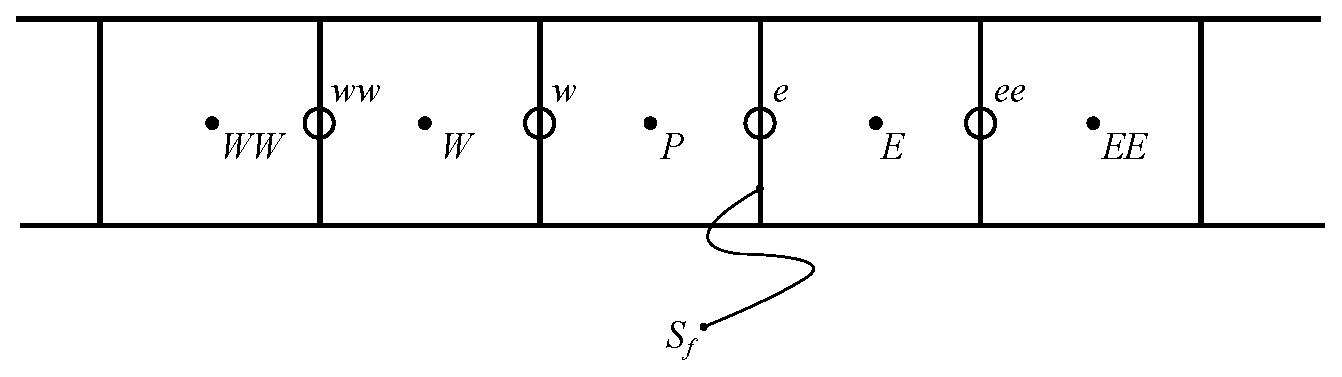
\includegraphics[width=0.7\textwidth]{fig/cells.eps}
    \caption{One-dimensional FVM discretization}
    \label{fig:4a}
\end{figure}

First, the Momentum Predictor (Eq. (\ref{eq:MOMPRED})) will be rewritten in terms of the errors in 1D as follows:

\begin{equation}
    \dfrac{a_P}{\omega} \; u_P^* + a_E \; u_E^* + a_W \; u_W^* = \dfrac{1-\omega}{\omega} \; a_P \; u_P^0 - (\hat{\nabla} p)_P + \Phi_P
\end{equation}

\begin{equation}
    \dfrac{a_P}{\omega} \; e_{u,P}^* + a_E \; e_{u,E}^* + a_W \; e_{u,W}^* = \dfrac{1-\omega}{\omega} \; a_P \; e_{u,P}^0 - \dfrac{S_f}{2} (e^0_{p,E}-e^0_{p,W})
    \label{eq:MPerror}
\end{equation}

\noindent where $P$, $W$ and $E$ represents the main cell and neighbour cells respectively on this current FVM stencil (see Fig. \ref{fig:4a}).

Now, the errors can be written in terms of the Fourier decomposition as:

\begin{equation}
    e^k_{\phi,M} = \alpha^k_{\phi} \; \text{exp} \left(i \; \dfrac{x_M \; \theta}{\Delta x}\right)
    \label{eq:error}
\end{equation}

\noindent which, for multivariable systems as the present one, it becomes:

\begin{equation}
\begin{bmatrix}
e_u \\
e_p 
\end{bmatrix}^{k}
=
\begin{bmatrix}
u \\
p 
\end{bmatrix}^{n+1}
-\begin{bmatrix}
u \\
p 
\end{bmatrix}^{k}
=
\begin{bmatrix}
\alpha_u \\
\alpha_p 
\end{bmatrix}^{k}
\; \text{exp}\left[ i \; \theta \; \frac{x_M}{\Delta x}\right]
\label{eq:fou1}
\end{equation}

Replacing each error on Eq. (\ref{eq:MPerror}) for its corresponding Fourier decomposition (as given by Eq. (\ref{eq:error})), the following equation is obtained:

\begin{equation}
    \left[ \dfrac{a_P}{\omega}  + a_E \; \text{exp} (i \theta) + a_W \; \text{exp} (-i \theta) \right] \alpha_u^* = \left( \dfrac{1-\omega}{\omega} \; a_P \right) \; \alpha_u^0 + \left(- \dfrac{S_f}{2} \right) \left(\text{exp} \left(i \; \theta \right) -  \text{exp} \left(-i \; \theta \right) \right) \alpha_p^0
    \label{eq:MPfou}
\end{equation}

\noindent where $P_u = \dfrac{a_P}{\omega}  + a_E \; \text{exp} (i \theta) + a_W \; \text{exp} (-i \theta)$, which leads to:

\begin{equation}
     \alpha_u^* = a_1 \alpha_u^0 + b_1 \alpha_p^0
    \label{eq:MPfou2}
\end{equation}

\noindent where:

\begin{equation}
\begin{split}
     a_1 &= \dfrac{1-\omega}{\omega} \; a_P \; P_u^{-1} \\
     b_1 &= - \left( \dfrac{S_f}{2} \right) \left( \text{exp} \left(i \; \theta \right) -  \text{exp} \left(-i \; \theta \right) \right) \; P_u^{-1}
\end{split}
\end{equation}

\noindent and since $p^* = p^0$, the following amplification system is obtained for the Momentum Predictor step:

\begin{equation}
\begin{bmatrix}
\alpha_u \\
\alpha_p 
\end{bmatrix}^{*} =
\begin{bmatrix}
a_1 & b_1 \\
0 & 1
\end{bmatrix}
\begin{bmatrix}
\alpha_u \\
\alpha_p 
\end{bmatrix}^{0} =
[A_1]
\begin{bmatrix}
\alpha_u \\
\alpha_p 
\end{bmatrix}^{0}
\end{equation}

This step of the algorithm, the Momentum Predictor, is the same for each one of the methods previously described. The next step, the Pressure Equation and Velocity Corrector, will differ for each algorithm so they will be presented separately. First, the SIMPLE algorithm with pressure relaxation will be presented, followed by the standard SIMPLEC and the current COMPLEX algorithms.

The pressure equation in terms of the errors for the SIMPLE algorithm is obtained from Eq. (\ref{eq:pEqnSIMPLE3}), which leads to:

\begin{equation}
    S_f (e_{p,E}^{**} - 2 e_{p,P}^{**} + e_{p,W}^{**}) = 
     -\left(\dfrac{a_E}{2}\right) (e_{u,EE}^* - e_{u,P}^*) 
    -\left(\dfrac{a_W}{2}\right) (e_{u,P}^* - e_{u,WW}^*)  +
    \left( \dfrac{1-\omega}{\omega} \right) \left(\dfrac{a_P}{2}\right) (e_{u,E}^0 - e_{u,W}^0)
\end{equation}

\noindent and the Fourier decomposition of the error (with pressure relaxation) becomes:

\begin{equation}
\begin{split}
    \alpha_p^{**} = &\left( \dfrac{\omega_p}{S_f \Sigma} \right) 
                    \left\{ \left(-\dfrac{a_E}{2} \right) \left[\text{exp} (2 i \theta) - 1 \right] +
                            \left(-\dfrac{a_W}{2} \right) \left[1 - \text{exp} (-2 i \theta)\right]
                    \right\} \alpha_u^{*} \\
                    & + \left( \dfrac{\omega_p}{S_f \Sigma} \right) 
                    \left\{ \left(\dfrac{1-\omega}{\omega} \right) \left(\dfrac{a_P}{2} \right) \left[\text{exp} (i \theta) - \text{exp} (- i \theta) \right] 
                    \right\} \alpha_u^{0} \\
                    & + (1-\omega_p) \alpha_p^*    
\end{split}
\end{equation}

\noindent where $\alpha_u^{**} = \alpha_u^{*}$.

\noindent and for the velocity corrector, the equation for the error may be written as:

\begin{equation}
    e_{u,P}^{***} = -\dfrac{\omega a_E}{a_P} e_{u,E}^{*} -\dfrac{\omega a_W}{a_P} e_{u,W}^{*} +
                   -\dfrac{\omega S_f}{2 a_P} (e_{p,E}^{**}-e_{p,W}^{**}) +
                   (1-\omega) \; e_{u,P}^0
\end{equation}

\noindent which, in Fourier factors, becomes:

\begin{equation}
    \alpha_{u}^{***} = \left[\left(-\dfrac{\omega a_E}{a_P}\right) \text{exp} (i \theta) + \left(- \dfrac{\omega a_W}{a_P}\right) \text{exp} (- i \theta)\right] \alpha_u^{**} +
                   \left\{\left(-\dfrac{\omega S_f}{2 a_P}\right) \left[\text{exp} (i \theta)-\text{exp} (-i \theta)\right] \right\} \alpha_p^{**} +
                   (1-\omega) \; \alpha_u^0
\end{equation}

\noindent with $\alpha_p^{***}=\alpha_p^{**}$.

Finally, the amplification of the sequence adding the pressure equation is:

\begin{equation}
\begin{bmatrix}
\alpha_u \\
\alpha_p 
\end{bmatrix}^{**} =
[A^S_2]
\begin{bmatrix}
\alpha_u \\
\alpha_p 
\end{bmatrix}^{*} +
[A^S_4]
\begin{bmatrix}
\alpha_u \\
\alpha_p 
\end{bmatrix}^{0} =
([A^S_2] [A_1] + [A^S_4])
\begin{bmatrix}
\alpha_u \\
\alpha_p 
\end{bmatrix}^{0}
\end{equation}

\noindent and, adding the velocity correction amplification contribution, the total amplification matrix ($A^S$) for the SIMPLE algorithm is given by:

\begin{equation}
\begin{bmatrix}
\alpha_u \\
\alpha_p 
\end{bmatrix}^{***} =
[A^S_3]
\begin{bmatrix}
\alpha_u \\
\alpha_p 
\end{bmatrix}^{**} +
[A^S_5]
\begin{bmatrix}
\alpha_u \\
\alpha_p 
\end{bmatrix}^{0} =
([A^S_3] [A^S_2] [A_1] + [A^S_3] [A^S_4] + [A^S_5])
\begin{bmatrix}
\alpha_u \\
\alpha_p 
\end{bmatrix}^{0} =
[A^S]
\begin{bmatrix}
\alpha_u \\
\alpha_p 
\end{bmatrix}^{0} 
\end{equation}

\noindent where:

\begin{equation}
[A^S_2]= 
\begin{bmatrix}
1 & 0 \\
c^S_2 & d^S_2
\end{bmatrix}
\; \; \; \; \; \;
[A^S_3]= 
\begin{bmatrix}
a^S_3 & b^S_3 \\
0 & 1
\end{bmatrix}
\; \; \; \; \; \;
[A^S_4]= 
\begin{bmatrix}
0 & 0 \\
c^S_4 & 0
\end{bmatrix}
\; \; \; \; \; \;
[A^S_5]= 
\begin{bmatrix}
a^S_5 & 0 \\
0 & 0
\end{bmatrix}
\end{equation}

\noindent and:

\begin{equation}
\begin{split}
     c^S_2 &= \left( \dfrac{\omega_p}{S_f \Sigma} \right) 
                    \left\{ \left(-\dfrac{a_E}{2} \right) \left[\text{exp} (2 i \theta) - 1 \right] +
                            \left(-\dfrac{a_W}{2} \right) \left[1 - \text{exp} (-2 i \theta)\right]
                    \right\} \\
     d^S_2 &= (1-\omega_p) \\
     a^S_3 &= \left[\left(-\dfrac{\omega a_E}{a_P}\right) \text{exp} (i \theta) + \left(- \dfrac{\omega a_W}{a_P}\right) \text{exp} (- i \theta)\right] \\
     b^S_3 &= \left\{\left(-\dfrac{\omega S_f}{2 a_P}\right) \left[\text{exp} (i \theta)-\text{exp} (-i \theta)\right] \right\} \\ 
     c^S_4 &= \left( \dfrac{\omega_p}{S_f \Sigma} \right) 
                    \left\{ \left(\dfrac{1-\omega}{\omega} \right) \left(\dfrac{a_P}{2} \right) \left[\text{exp} (i \theta) - \text{exp} (- i \theta) \right] 
                    \right\} \\
     a^S_5 &= (1-\omega)      
\end{split}
\end{equation}

For each method, the total amplification matrix is always defined as the product of the matrices of each step following the rule:

\begin{equation}
[A^m] = ([A^m_3] [A^m_2] [A_1] + [A^m_3] [A^m_4] + [A^m_5])
\end{equation}

\noindent where the superscript $m$ indicates the coupling method being considered ($S$ for SIMPLE, $C$ for SIMPLEC and $X$ for COMPLEX).

Looking at Eqs. (\ref{eq:pEqnSIMPLEC2}) and (\ref{eq:uCorrSIMPLEC}), and taking into account the relation between $\nabla p_P^*$ and the velocity field after the momentum predictor given by Eq. (\ref{eq:MOMPRED}), the amplification of the error during the pressure equation resolution and the velocity corrector step of SIMPLEC have a few differences compared to the SIMPLE amplification matrices in the following elements:

\begin{equation}
\begin{split}
     c^C_2 &= c_2^S + \left(\dfrac{a_E + a_W}{2}\right) [\text{exp} (i    \theta) - \text{exp} (-i \theta)] \\
     d^C_2 &= 1 \\
     a^C_3 &= \left(\dfrac{a_P}{\omega \tilde{a}_P}\right) a_3^S + \dfrac{a_E+a_W}{\tilde{a}_P} \\
     b^C_3 &= \left(\dfrac{a_P}{\omega \tilde{a}_P}\right) b_3^S \\ 
     c^C_4 &= \dfrac{1}{\omega_P} c^S_4 \\
     a^C_5 &= \left(\dfrac{a_P}{\omega \tilde{a}_P}\right) a^S_5     
\end{split}
\end{equation}

The same procedure may be applied for the COMPLEX method based on Eqs. (\ref{Eq:complexSemiFinal}) and (\ref{eq:uPrimeCOMPLEX}). Here it should be noticed that the issue regarding the definition of the gradient of the velocity correction $\nabla \boldsymbol{u}_P'$ using a single unknown scalar value $\alpha$, is no longer an issue for one-dimensional problems. Eq. (\ref{eq:gradApprox}) now provides mathematical closure for the problem with no assumption needed, since the gradient of a vector field in 1D is, in fact, a scalar value. The amplification matrix elements for COMPLEX now become:

\begin{equation}
\begin{split}
     c^X_2 = c_2^C &+ \left(\dfrac{a_E}{8}\right) \left[\text{exp} (3 i \theta) + \text{exp} (2 i \theta) - 2 \text{exp} (i \theta) - 2 + \text{exp} (-i \theta) + \text{exp} (-2 i \theta)\right] \\
     &+ \left(-\dfrac{a_W}{8}\right) \left[\text{exp} (2 i \theta) + \text{exp} (i \theta) - 2 - 2 \text{exp} (-i \theta) + \text{exp} (-2 i \theta) + \text{exp} (-3 i \theta)\right] \\
     d^X_2 = d^C_2& \\
     a^X_3 = a^C_3 &+ \left(\dfrac{a_E}{4}\right) \left[\text{exp} (2 i \theta) + \text{exp} (i \theta) - 1 - \text{exp} (-i \theta) \right] \\
     &+ \left(-\dfrac{a_W}{4}\right) \left[\text{exp} (i \theta) + 1 - \text{exp} (- i \theta) - \text{exp} (-2 i \theta) \right] \\
     b^X_3 = b_3^C& \\ 
     c^X_4 = c^C_4& \\
     a^X_5 = a^C_5&     
\end{split}
\end{equation}

The von Neumann stability criteria \cite{hirsch} will be applied to determine the range of stability of each method. This criteria for multivariable problems may be expressed as:

\begin{equation}
\beta(\theta) = \text{max}_i \{ |\lambda_i(\theta)| \} \leq 1
\label{eq:AmpCrit}
\end{equation}

\noindent where $\beta$ is the amplification factor and $\lambda$ are the eigenvalues of the amplification matrix $[A^m]$. If Eq. (\ref{eq:AmpCrit}) is fulfilled, then the method will be considered numerically stable (under the hypothesis of the Fourier analysis). Moreover, the value of $\beta$ gives a notion about the convergence rate of the method (i.e. if the values are below but close to unity, then the method will probably have a slow convergence rate, while the opposite happens when the values are close to zero).

Fig. (\ref{fig:1a}) shows the amplification factor for each method with a relaxation factor $\omega=0.7$ ($\omega_p=1-\omega$ for SIMPLE) for low and high mesh-Reynolds numbers ($Re_h = \dfrac{h U}{\nu}$). It is observed that SIMPLE has always a higher amplification factor (slower convergance rate) for each frequency and for each $Re_h$ considered. On the other hand, the SIMPLEC method gets slightly affected with the change of $Re_h$ while COMPLEX does not show any significant variation. All methods show a stable behavior under the Fourier conditions, while COMPLEX and SIMPLEC show lower amplification factors than SIMPLE. 

\begin{figure}[H]
    \centering
    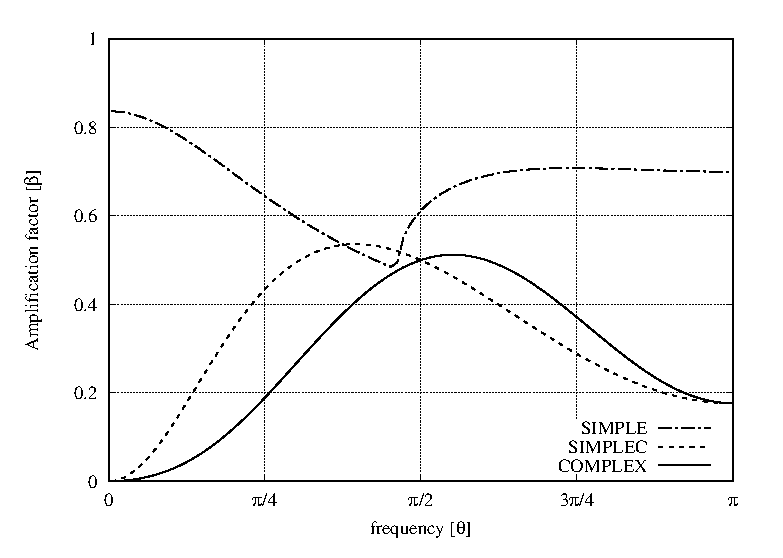
\includegraphics[width=0.45\textwidth]{fig/Re0001} \hspace{1cm}
    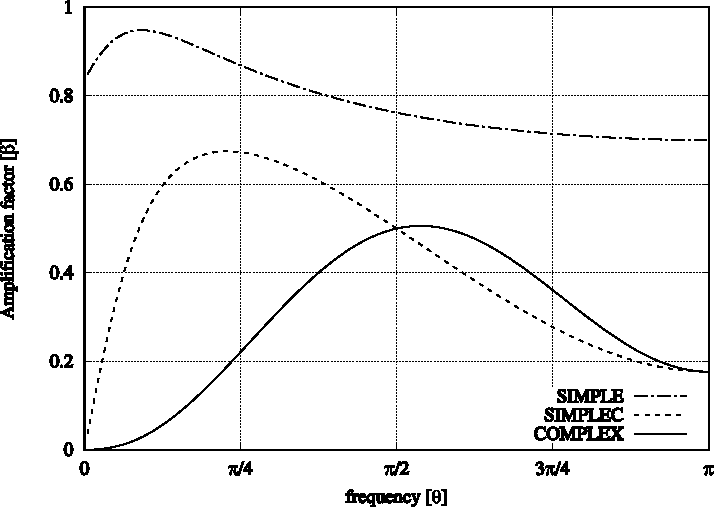
\includegraphics[width=0.45\textwidth]{fig/Re1000}
    \caption{Amplification factor for $Re_h=0.001$ (left) and $Re_h=1000$ (right)}
    \label{fig:1a}
\end{figure}
    
Fig. (\ref{fig:1b}) shows the sensitivity of the amplification factor to the momentum relaxation factor for all frequencies and for the three coupling methods. The results are obtained for a $Re_h=1$ and always considering the rule $\omega_P = 1 - \omega$ for SIMPLE. While the SIMPLE algorithm does not show any significant improvement for higher values of $\omega$ (even showing a range of instability for low frequencies at $\omega=0.95$ and $\omega_P=0.05$), the SIMPLEC algorithm shows a depletion in its performance for reducing errors of low frequency with high momentum relaxation factors (tending to unity for $\theta=0$ as $\omega \rightarrow 1$). In this aspect, the COMPLEX algorithm shows a clear advantage over the other two methods by maintaining almost unaltered the overall error damping, even for high momentum relaxation factors.     
    
\begin{figure}[H]
    \centering
    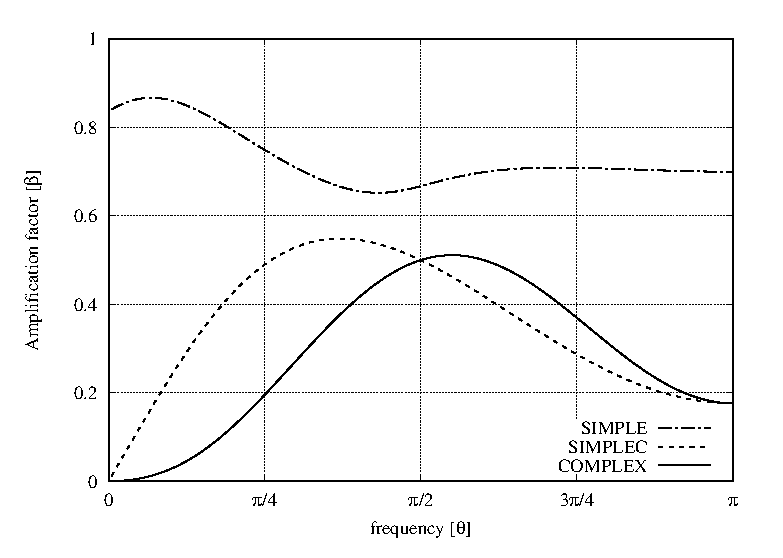
\includegraphics[width=0.45\textwidth]{fig/w07} \hspace{1cm}
    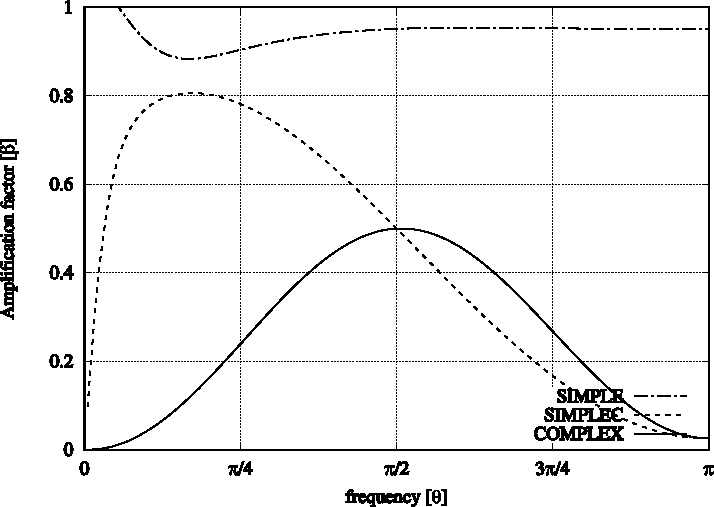
\includegraphics[width=0.45\textwidth]{fig/w095}
    \caption{Amplification factor for $\omega=0.7$ (left) and $\omega=0.95$ (right)}
    \label{fig:1b}
\end{figure}    

This theoretical advantage (always considering the hyphothesis of the Fourier analysis and one-dimensional problems) is very important since it indicates that the good performance of the method holds up even when the convergence rate to the steady state solution is accelerated by increasing the momentum relaxation factors. In the next section, this advantage will be put to the test for two benchmark tridimensional problems to see how accurate are the a-priori predictions of the Fourier techniques on real CFD problems.

The analysis of the sensitivity to the momentum relaxation factor may be deepened by considering a continuous range as relaxation factors from $0$ to $1$ for the three methods, as shown in Figs. \ref{fig:1c1}, \ref{fig:1c2} and \ref{fig:1c3}. These figures show a clear advantage of SIMPLEC over SIMPLE for almost every relaxation factor considered, and a clear advantage of COMPLEX over SIMPLE for high values of the amplification factor. Here it may be noted that, for very low values of $\omega$ all methods tend to the same stability behavior.

\begin{figure}[H]
    \centering
    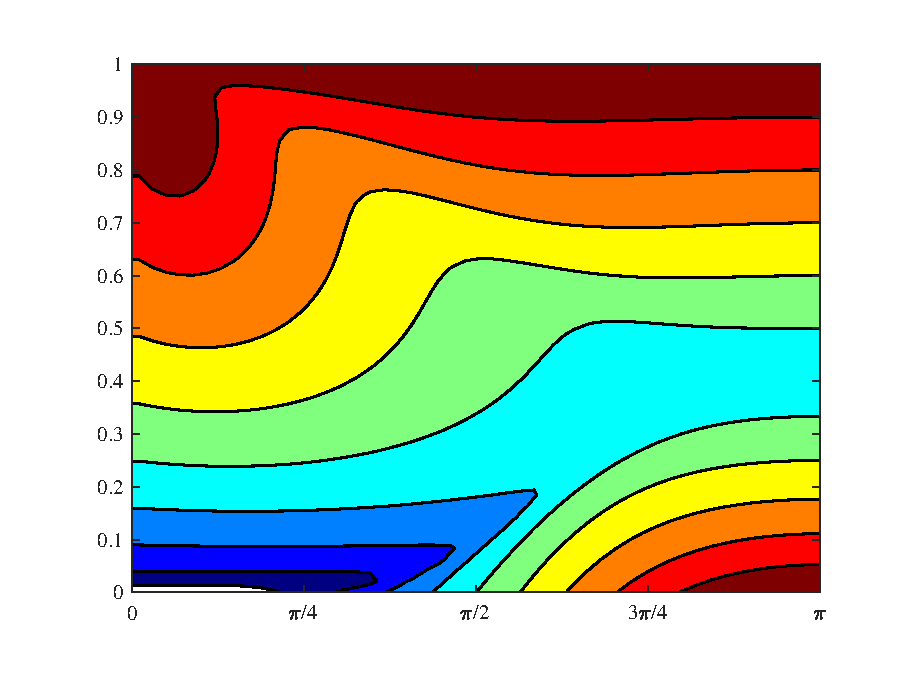
\includegraphics[width=0.6\textwidth]{fig/SIMPLE_map}
    \caption{Amplification factor for SIMPLE for different relaxation factors and frequencies}
    \label{fig:1c1}
\end{figure}  
\begin{figure}[H]
    \centering    
    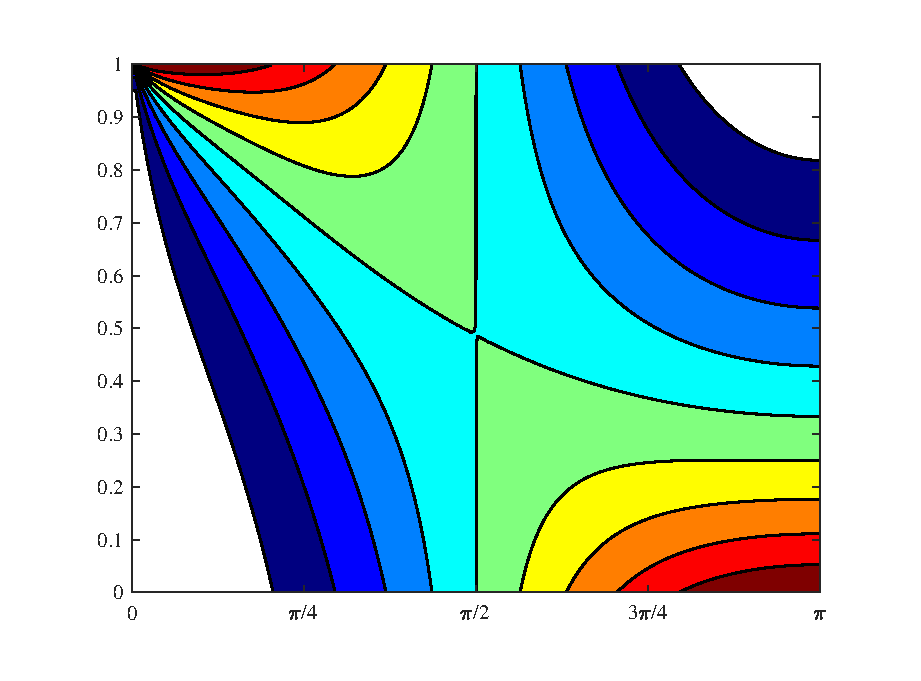
\includegraphics[width=0.6\textwidth]{fig/SIMPLEC_map}
    \caption{Amplification factor for SIMPLEC for different relaxation factors and frequencies}
    \label{fig:1c2}
\end{figure}  
\begin{figure}[H]
    \centering           
    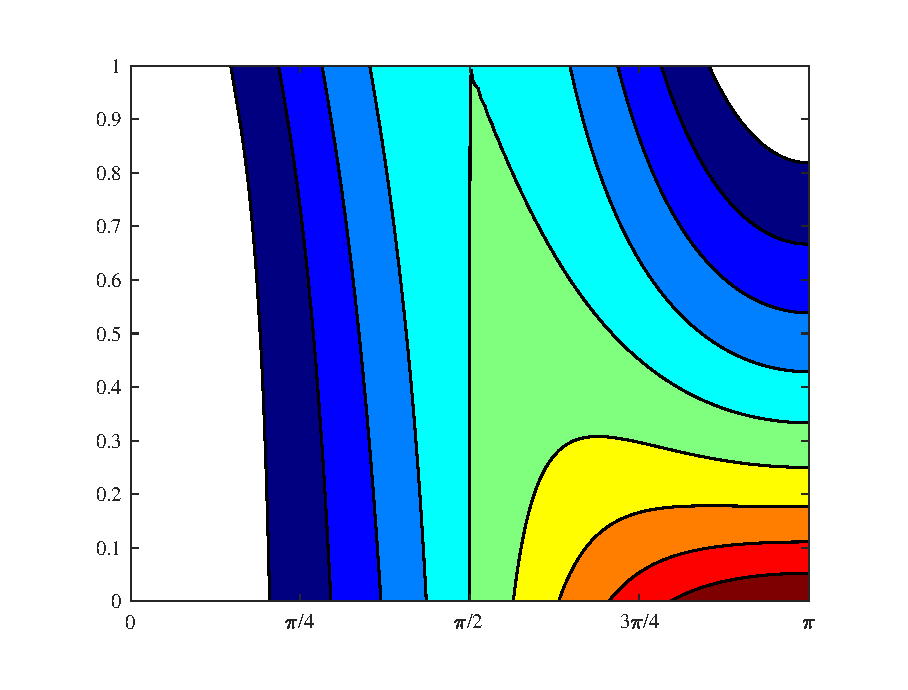
\includegraphics[width=0.6\textwidth]{fig/COMPLEX_map}
    \caption{Amplification factor for COMPLEX for different relaxation factors and frequencies}
    \label{fig:1c3}
\end{figure}    
    
A method to quantify the overall error damping for a general problem, where the initial solution is formed by an equally distributed amount of modes (i.e. there is no frequency that is clearly dominant over the others in the initial values of $u$ and $p$ fields), is to consider an average amplification factor over all the frequencies. This is shown in Fig. \ref{fig:1d}, where the mean value of $\beta$ over all frequencies is plotted for all the possible values of the momentum relaxation factors. Here it is also clear that, while all methods are stable under these conditions, the SIMPLEC and COMPLEX algorithms are clearly more efficient in terms of the error damping, and the COMPLEX algorithm outperforms SIMPLEC when the relaxation factor is increased. 

\begin{figure}[H]
    \centering
    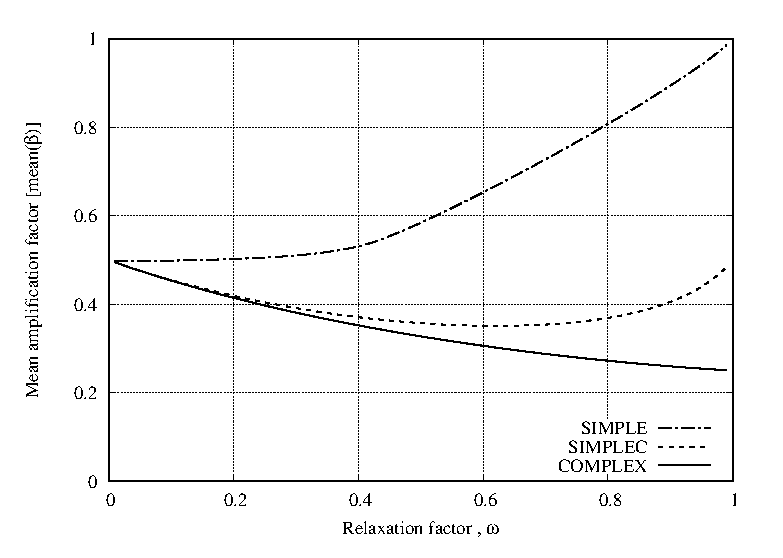
\includegraphics[width=0.6\textwidth]{fig/meanAmp}
    \caption{Mean amplification factor for each relaxation of momentum $\omega$}
    \label{fig:1d}
\end{figure}  

\section{Test cases}
\label{sec:cases}

In this section, the new pressure-velocity coupling strategy is analysed in the context of incompressible, laminar and stationary Newtonian flows. On this line, the numerical performance of the method is compared with  SIMPLE and SIMPLEC by evaluating the total number of iterations required to achieve a convergence criteria. First of all, the details of each problem are explained followed by the definition of the convergence criteria. Subsequently, the numerical configuration of the simulations are commented and after that, two different analysis over the COMPLEX method are performed. On the one hand, a serie of simulations are carried out to investigate a suitable value of the complex factor $\kappa$ and finally, a comparison of the current proposal with SIMPLE and SIMPLEC is presented for various conditions. 

\subsection{Test problems}\label{Section:problemDescription}
 The evaluation of the COMPLEX method is achieved by solving two typical tests for incompressible and stationary flows. The first of them is the cubic cavity test and the second one is the flow through the Backward Facing Step (BFS) channel.
\subsubsection{Cavity}
 A graphical scheme of this problem is depicted in Fig.~\ref{Fig:Cavity}.
\begin{figure}[t!]
\centering
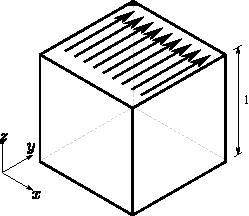
\includegraphics[width=5cm]{fig/Cases/Cavity.pdf}
\caption{The cubic cavity problem where a fixed tangential velocity is imposed on the upper face.}
\label{Fig:Cavity}
\end{figure} 
There, a tangential fixed velocity of 1 m/s is imposed on the upper face of the cubic domain of length 1 m. The case is solved using to different values of the kinematic viscosity, $\nu = 2.5\, e-3$ m$^2$/s and $\nu = 2.5$ m$^2$/s which defines the Reynolds number of 400 and $0.4$ respectively. For the purposes of this paper, the cavity is discretised with hexahedral cells using three different refinement levels: a coarse mesh with 25 divisions per side (15625 cells), a medium mesh with 50 divisions per side (125000 cells) and a fine mesh with 100 divisions per side (1000000 cells).

\subsubsection{Backward Facing Step}
The domain of this test and its dimension are shown in Fig.~\ref{Fig:Geometria3}.
\begin{figure}[b!!!!]
\centering
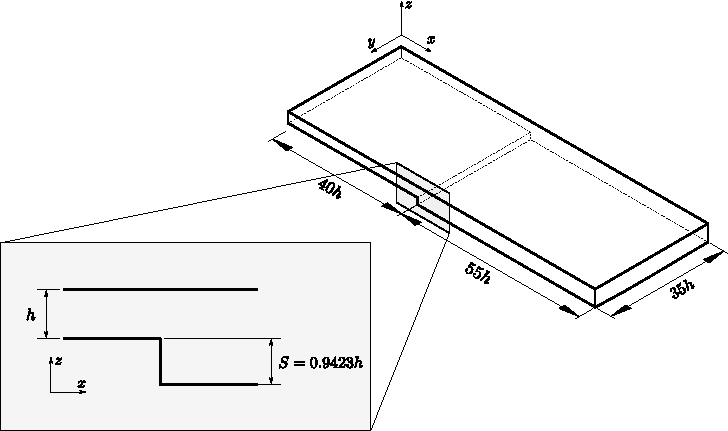
\includegraphics[width=12cm]{fig/Cases/Geometria3.pdf}
\caption{Description of the BFS domain where the dimensions are defined relative to the inlet height $h = 1$ m.}
\label{Fig:Geometria3}
\end{figure}
At the inlet, a constant and normal velocity of 1 m/s of magnitude is set up. Analogously to the cavity case, the problem is simulated with two different viscosity values, $\nu = 5.141\,e-3$ m$^2$/s and $\nu = 5.141$ m$^2$/s which refers to the Reynolds number of 389 and $0.389$ respectively. The BFS is discretized with hexahedral cells using three different mesh sizes as defined in Table~\ref{Table:BFSMeshes} with a variable cell size as plotted in Fig.~\ref{Fig:Factores} where the near wall regions and the step sector are relatively refined.
\begin{table}[b!]
\centering
\begin{tabular}{cccccccc}
\hline 
\multirow{2}{1cm}{Mesh Level} & \multicolumn{3}{c}{Pre-step divisions} & \multicolumn{3}{c}{Post-step divisions} & \multirow{2}{1cm}{Total Cells} \\ 
\cline{2-7} 
&  $x-$axis &  $y-$axis &  $z-$axis &  $x-$axis &  $y-$axis &  $z-$axis \\ 
\hline 
Coarse & 20 & 40 & 8 & 26 & 40 & 16 & 23040 \\ 
Medium & 40 & 80 & 15 & 52 & 80 & 30 & 172800 \\ 
Fine & 80 & 160 & 30 & 104 & 160 & 60 & 1382400 \\ 
\hline 
\end{tabular}
\caption{Scheme of divisions for the BFS case. The pre-step and post-step are the upstream and downstream regions of the step transversal section.}
\label{Table:BFSMeshes}
\end{table}

\begin{figure}[t!!!]
\centering
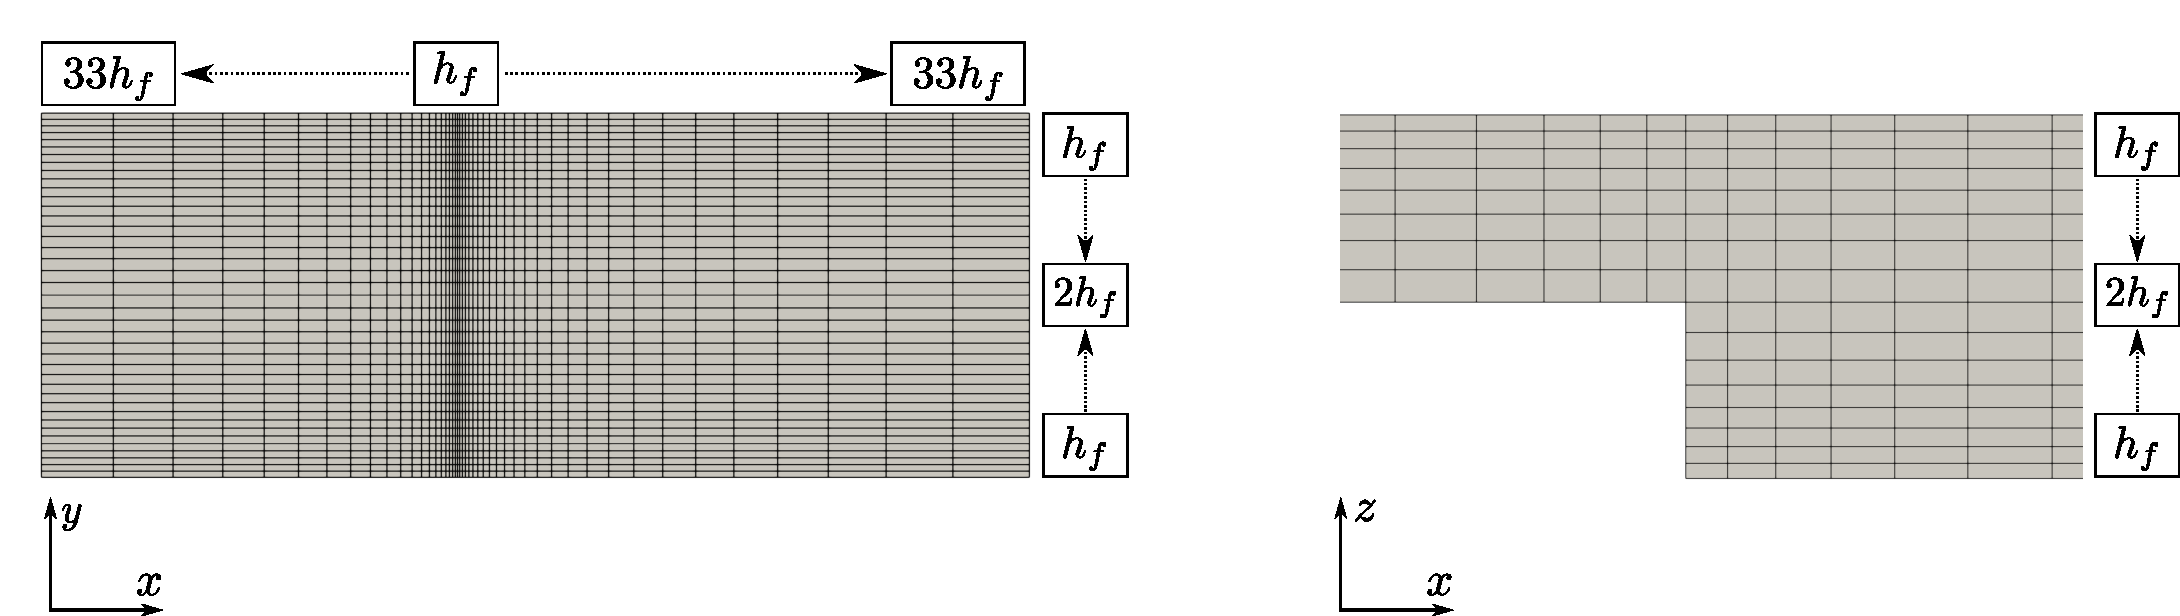
\includegraphics[width=16cm]{fig/Cases/Factores.pdf}
\caption{Variable cell refinement in the BFS.  On the left figure, the cell size grows from the step point up to the inlet and outlet boundaries and from the lateral walls up to the middle longitudinal section. On the right, the cell size in the post-step regions grows from the bottom and upper walls up to the middle height section of the channel.}
\label{Fig:Factores}
\end{figure}

\subsection{Error measurement}
To analyse the rate of convergence of the different algorithms, an error measure is defined. The error is assumed to be the residual of the discretized Navier-Stokes equations which are computed for each cell $P$ of the FV mesh $\Omega$. Then, the momentum residual writes,
\begin{equation}
\label{Eq:R1Discretized}
R_1(P)
=
\sum_{f}
\varphi_f\,
\boldsymbol{u}_p
+
\nu
\sum_f
\nabla \boldsymbol{u}_f
\cdot
\boldsymbol{S}_f
+
\sum_f
p_f
\,
\boldsymbol{S}_f
-
\boldsymbol{\Phi}_P \, V_P
\qquad \qquad
\forall P\,\in\,\Omega,
\end{equation}
and analogously, the mass residual may be computed as follows,
\begin{equation}
R_2(P)
=
\sum_f
\boldsymbol{u}_f
\cdot
\boldsymbol{S}_f
\qquad \qquad
\forall P\,\in\,\Omega,
\end{equation}
where the face velocity value $\boldsymbol{u}_f$ is replaced in terms of the momentum equation such as done in Eq.~(\ref{Eq:firstPressureEq}),
\begin{equation}
\label{Eq:R2Discretized}
R_2(P)
=
\sum_f 
\left(
\frac{1}{a_P}
\right)_f 
\nabla p_f
\cdot
\boldsymbol{S}_f 
-
\sum_f
\left(
\frac{\boldsymbol{H}}
{a_P}
\right)_f 
\cdot 
\boldsymbol{S}_f,
\qquad \qquad
\forall P\,\in\,\Omega.
\end{equation}
It is important to highlight that the computations of $R_1$ and $R_2$ are independent of the pressure-velocity coupling strategy employed. These equations are only function of the velocity and pressure values, and of the momentum equation coefficients which are equally assembled for the three pressure-velocity coupling methods studied in this paper. In addition to this, the residuals $R_1$ and $R_2$ are computed at the end of each time step of the simulation. 
On the basis of their definition, the residuals $R_1$ and $R_2$ are an appropriate indicator to qualify the convergence of the different numerical algorithms by isolating their specific influence. In particular of this paper, the Root Mean Square (RMS) value of them is computed, 
\begin{align}
\overline{R}_1
&=
\sqrt
{
\sum_{P\,\in\,\Omega}
R_1(P)^2
}
\\
\overline{R}_2
&=
\sqrt
{
\sum_{P\,\in\,\Omega}
R_2(P)^2
}.
\end{align}
Referring to the $\overline{R}_1$ and $\overline{R}_2$, the following convergence criteria is proposed in this work: a numerical simulation will be assumed as converged if both values, $\overline{R}_1$ and $\overline{R}_2$  are below a tolerance of $1e^{-9}$,
\begin{equation}
\label{Eq:convergenceCriteria}
\left\lbrace
\begin{array}{c}
\overline{R}_1 \leq 1e^{-9} \\
\overline{R}_2 \leq 1e^{-9}
\end{array}
\right..
\end{equation}

\subsection{Numerical setup}
The simulations of the different analysis are configured with the same numerical schemes. Namely, the convective terms are discretised with an upwind scheme and the pressure gradient operator is computed with a Gauss-based formula using linear interpolation to define the face values. Respecting the diffusive terms, they are discretized with a Gauss-based formula where the face gradient is assembled with a first-neighbour stencil. The linear system of equations are solved until a convergence of two order of magnitude is achieved for both, the momentum and mass balance systems. 

With reference to the relaxation factors, the momentum relaxation factor $\omega_u$ is a variable of the parametric study. On the other side, the pressure relaxation $\omega_p$ is equal to one in the COMPLEX and SIMPLEC simulations and in the SIMPLE ones it is defined as follows,
\begin{equation}
\label{Eq:relaxP}
\omega_p = 1 - \omega_u.
\end{equation}

  

\subsection{Study of the complex factor $\kappa$}
An important parameter of the current numerical method is the complex factor $\kappa$. In this study, the influence  of $\kappa$ on the convergence rate is analysed in combination with the relaxation factor for the momentum equation $\omega_{u}$ where the number of iterations required to reach the convergence criteria of Eq.~(\ref{Eq:convergenceCriteria}) is quantified.

The study solves a serie of simulations of the cavity and BFS problems using the medium refinement levels of the proposed meshes respectively. Furthermore, for each case, two different physical configuration are addressed according to the two Reynolds number proposed. Consequently, four different numerical problems are defined. Each one of this four simulations is solved varying the values of $\kappa$ and $\omega_{u}$. The complex factor is ranged from 0 to 1 by a step of $0.05$ (21 values) and the relaxation factor from 0.8 up to 1 by a step of $0.1$ (21 values) respectively. In combination, this parametric study is composed by 441 simulations for each one of the four numerical problems.

The results of the simulations are presented in the Tables~\ref{Table:Cavity_LowRe}, \ref{Table:BFS_LowRe}, \ref{Table:Cavity_HighRe} and \ref{Table:BFS_HighRe}, and in the Fig.~\ref{Fig:FactorLowRe}. One one hand, the tables present the required number of iterations to reach the convergence as function of $\omega_u$ and $\kappa$. Not all simulations are displayed due to space limitations, the range of $\omega_u$ is shortened from 0.92 to 1 and the $\kappa$ values are listed using a step of 0.1 instead of 0.05. On the other hand, the Fig.~\ref{Fig:FactorLowRe} present the results of the four cases using contour plots. There is one figure per case which plots the relative number of iterations ($RI$) required for each simulation compared with those required for the simulation with the same relaxation factor but with $\kappa = 0$. Formally, the relative iteration index $RI$ for a given pair of values $\omega_u$ and $\kappa$ is computed as follows,
\begin{equation}
\label{Eq:relativeIndex}
RI(\omega_u, \kappa)
=
\dfrac
{
NI(\omega_u, \kappa) - NI(\omega_u, 0)
}
{
NI(\omega_u, 0)
}
\times
100 \%,
\end{equation}
where $NI(\omega_u, \kappa)$ is the number of iterations required for convergence using the relaxation value $\omega_u$ and the complex factor $\kappa$ and $NI(\omega_u, 0)$ is the number of iterations required for the convergence using the relaxation value $\omega_u$ and a complex factor equal to $\kappa = 0$.

\begin{table}[t!]
\centering
\begin{tabular}{c|ccccccccccc}
\hline 
$\omega_u$/$\kappa$ & 0 & 0.1 & 0.2 & 0.3 & 0.4 & 0.5 & 0.6 & 0.7 & 0.8 & 0.9 & 1 \\ 
\hline 
1 & div & div & div & div & div & div & div & div & div & div & div \\ 
0.99 & 1993 & 1702 & 1742 & 1754 & 1747 & 1742 & 1761 & div & div & div & div \\ 
0.98 & 991 & 842  & 845 & 856 & 866 & 870 & 870 & 868 & 865 & 863 & 864 \\ 
0.97 & 658 & 551  & 559 & 560 & 565 & 570 & 574 & 575 & 575 & 575 & 573 \\ 
0.96 & 491 &425  & 414 & 416 & 418 & 421 & 424 & 426 & 427 & 428 & 428 \\ 
0.95 & 391 & 348 & 327 & 330 & 332 & 333 & 335 & 337 & 338 & 339 & 339 \\ 
0.94 & 373 & 373 & 373 & 373 & 373 & 373 & 373 & 373 & 373 & 373 & 373 \\ 
0.93 & 438 & 438 & 438 & 438 & 438 & 438 & 438 & 438 & 438 & 438 & 438 \\ 
0.92 & 504 & 504 & 504 & 504 & 504 & 504 & 504 & 504 & 504 & 504 & 504 \\ 
\hline 
\end{tabular} 
\caption{Required number of iterations at convergence for the Cavity case with Re = $0.4$}
\label{Table:Cavity_LowRe}
\end{table}
\begin{table}[t!]
\centering
\begin{tabular}{c|ccccccccccc}
\hline 
$\omega_u$/$\kappa$ & 0 & 0.1 & 0.2 & 0.3 & 0.4 & 0.5 & 0.6 & 0.7 & 0.8 & 0.9 & 1 \\ 
\hline 
1 & div & div & div & div & div & div & div & div & div & div & div \\ 
0.99 & 1974 & 1697 & 1753 & 1865 & 1941 & 1993 & div & div & div & div & div \\ 
0.98 & 981 & 816 & 844 & 854 & 874 & 904 & 929 & 949 & 966 & 980 & 992 \\ 
0.97 & 651 & 528 & 550 & 560 & 565 & 571 & 581 & 594 & 606 & 618 & 627 \\ 
0.96 & 486 & 392 & 403 & 413 & 418 & 421 & 424 & 428 & 435 & 442 & 449 \\ 
0.95 & 387 & 320 & 317 & 324 & 330 & 333 & 335 & 336 & 339 & 342 & 346 \\ 
0.94 & 320 & 272 & 259 & 266 & 271 & 274 & 276 & 277 & 278 & 280 & 282 \\ 
0.93 & 273 & 237 & 220 & 225 & 229 & 232 & 234 & 235 & 236 & 237 & 238 \\ 
0.92 & 240 & 233 & 233 & 233 & 233 & 233 & 233 & 233 & 233 & 233 & 233 \\ 
\hline 
\end{tabular}
\caption{Required number of iterations at convergence for the BFS case with Re = 0.389}
\label{Table:BFS_LowRe}
\end{table}
\begin{table}[t!]
\centering
\begin{tabular}{c|ccccccccccc}
\hline 
$\omega_u$/$\kappa$ & 0 & 0.1 & 0.2 & 0.3 & 0.4 & 0.5 & 0.6 & 0.7 & 0.8 & 0.9 & 1 \\ 
\hline 
1 & div & div & div & div & div & div & div & div & div & div & div \\ 
0.99 & 1611 & 1321 & 1286 & 1333 & 1357 & div & div & div & div & div & div \\ 
0.98 & 802 & 693 & 652 & 635 & 648 & 662 & 671 & 678 & 682 & div & div \\ 
0.97 & 532 & 471 & 448 & 431 & 423 & 427 & 435 & 441 & 446 & 449 & 452 \\ 
0.96 & 398 & 357 & 342 & 330 & 321 & 317 & 319 & 323 & 327 & 331 & 333 \\ 
0.95 & 318 & 288 & 277 & 269 & 262 & 257 & 255 & 256 & 258 & 261 & 263 \\ 
0.94 & 266 & 243 & 235 & 229 & 225 & 221 & 218 & 216 & 215 & 216 & 217 \\ 
0.93 & 239 & 225 & 218 & 214 & 211 & 211 & 211 & 210 & 210 & 210 & 209 \\ 
0.92 & 243 & 243 & 242 & 242 & 242 & 241 & 241 & 241 & 241 & 241 & 240 \\ 
\hline 
\end{tabular}
\caption{Required number of iterations at convergence for the Cavity case with Re = 400}
\label{Table:Cavity_HighRe}
\end{table}
\begin{table}[t!]
\centering
\begin{tabular}{c|ccccccccccc}
\hline 
$\omega_u$/$\kappa$ & 0 & 0.1 & 0.2 & 0.3 & 0.4 & 0.5 & 0.6 & 0.7 & 0.8 & 0.9 & 1 \\ 
\hline 
1 & div & div & div & div & div & div & div & div & div & div & div \\ 
0.99 & div & div & div & div & div & div & div & div & div & div & div \\ 
0.98 & 818 & 624 & 632 & 637 & div & div & div & div & div & div & div \\ 
0.97 & 540 & 427 & 422 & 428 & 435 & div & div & div & div & div & div \\ 
0.96 & 403 & 329 & 323 & 327 & 329 & 478 & 3086 & div & div & div & div \\ 
0.95 & 322 & 272 & 264 & 266 & 268 & 351 & 712 & 4714 & div & div & div \\ 
0.94 & 269 & 236 & 227 & 226 & 250 & 320 & 483 & 1151 & div & div & div \\ 
0.93 & 240 & 225 & 218 & 221 & 246 & 299 & 397 & 608 & 1427 & div & div \\ 
0.92 & 242 & 235 & 230 & 232 & 256 & 292 & 351 & 457 & 696 & 1087 & 8863 \\ 
\hline 
\end{tabular}
\caption{Required number of iterations at convergence for the BFS case with Re = 389}
\label{Table:BFS_HighRe}
\end{table}
\begin{figure}[t!]
\centering
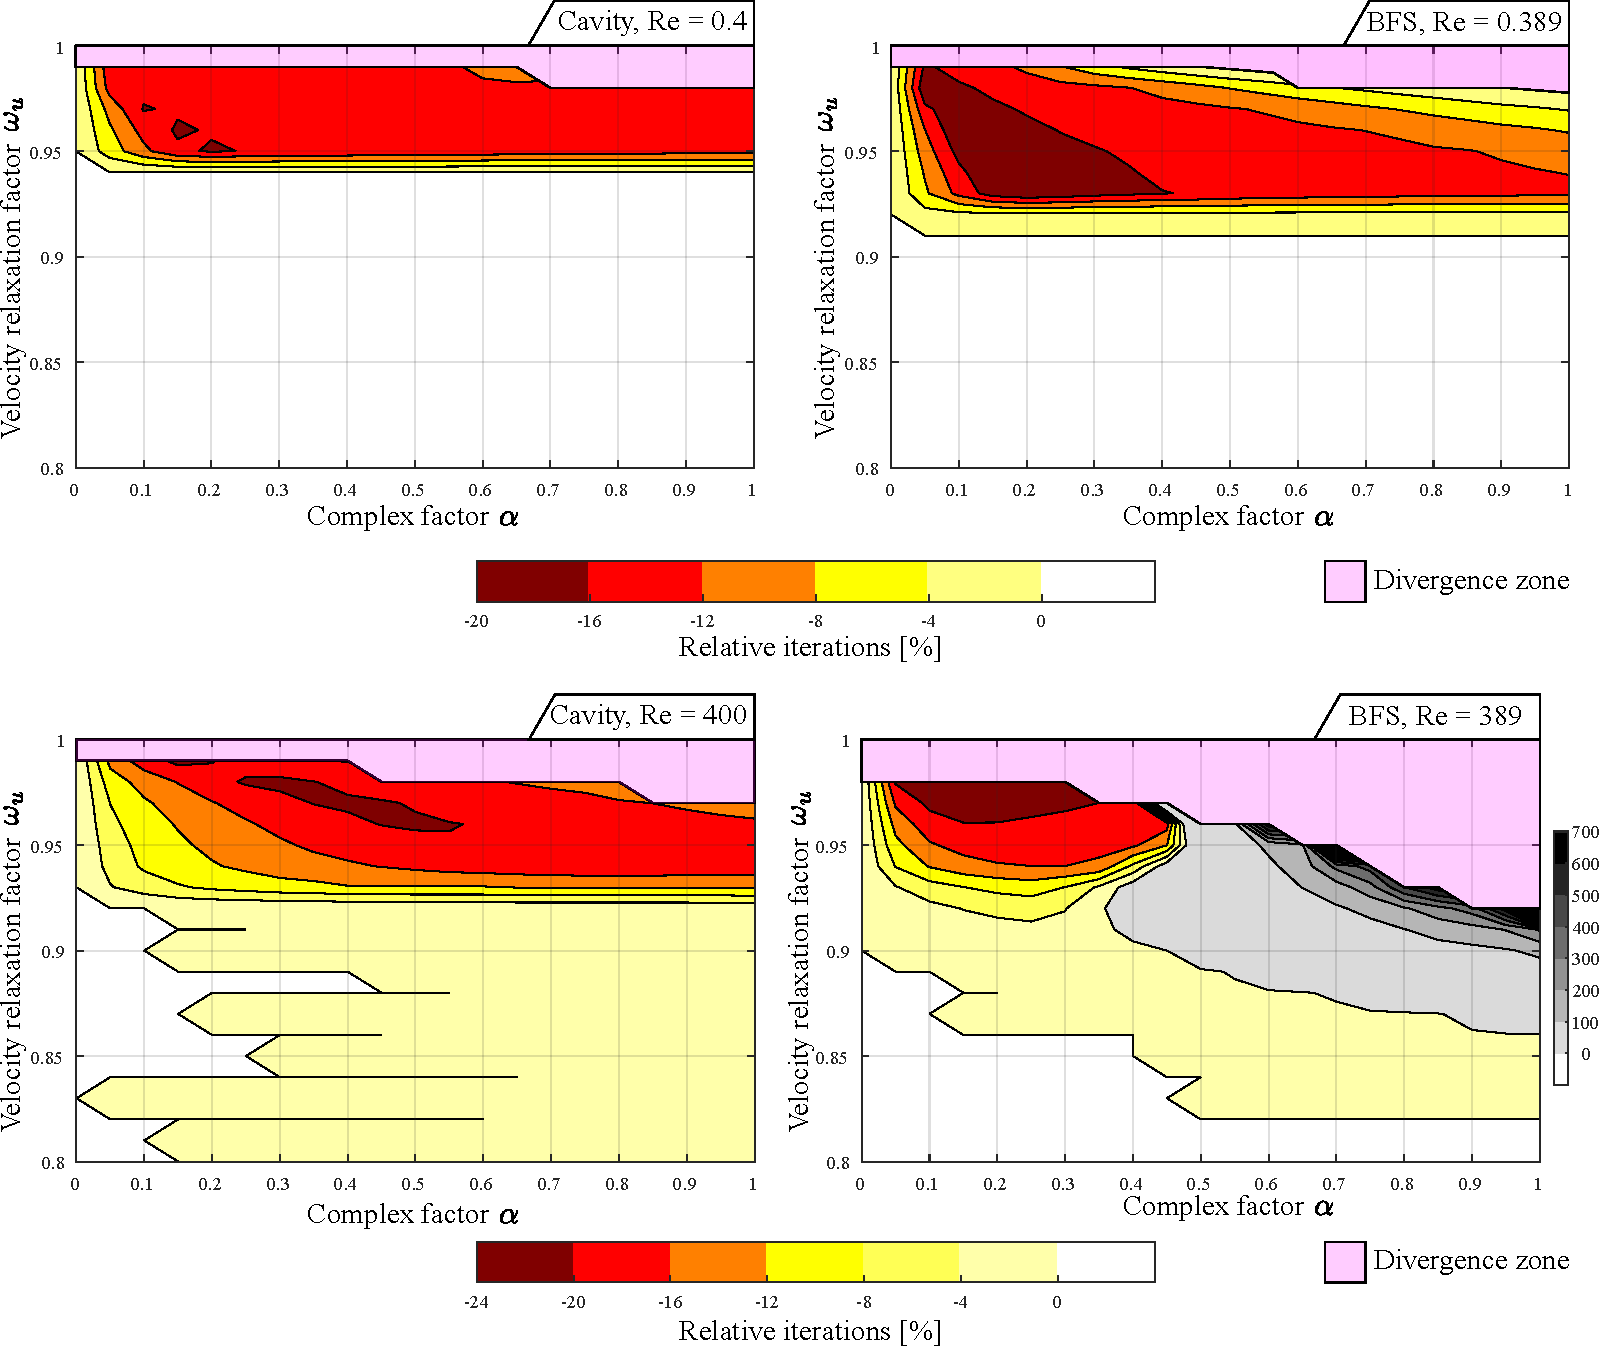
\includegraphics[width=17cm]{fig/Results/FactorLowRe.pdf}
\caption{Isolines of relative iterations as function of the momentum relaxation factor and the complex factor for the Cavity and BFS cases and the values of the Reynolds number employed respectively.}
\label{Fig:FactorLowRe}
\end{figure}
The Tables~\ref{Table:Cavity_LowRe},~\ref{Table:BFS_LowRe}, and the upper plots of Fig.~\ref{Fig:FactorLowRe} present the relative low Reynolds simulation results  and the Tables~\ref{Table:Cavity_HighRe},~\ref{Table:BFS_HighRe}, and the bottom plots of Fig.~\ref{Fig:FactorLowRe} present the relative high Reynolds ones. In general, it is concluded that the addition of the complex term does not influence the convergence when using relative low relaxation factors. On the contrary, with relative high values of $\omega_u$, the addition of the complex term reduces the number of iterations required for convergence. This reduction has a maximum value of approximately 20 $\%$ in the total number of iterations. The better results are obtained with values of the complex factor that are below $k = 0.5$. The simulations with high values of the complex factor $(k \geq 0.5)$ may be unstable. In particular, the BFS problem at Re = 389 indicates an extended divergence zone for the highest values of $\omega_u$ which is followed by a slow convergence zone (grey-coloured zone in the figure) for lower values of $\omega_u$. Unlike this last behavour, with lower values of $\kappa$, the simulations are stable and indicate the maximum convergence speed. 

In view of this investigation, it is concluded that a complex factor equal to $\kappa = 0.2$ is adequate to speed up the convergence without losing stability. This last inference is determined based on two different numerical problems (Cavity and BFS) in the range of Reynolds number between $0.4$ and $400$. 

 
\subsection{Comparison of COMPLEX with SIMPLE and SIMPLEC}
In the next paragraphs, a comparison of the COMPLEX strategy against the SIMPLE and SIMPLEC methods is performed. Here, the COMPLEX	 simulations are solved using a complex factor of $\kappa = 0.2$. 
Similar as solved in the previous section, the number of iterations required to reach the convergence criteria is measured. Each of the four numerical cases defined in previous section is solved using the coarse, medium and fine mesh levels. As well as the Reynolds number and the mesh refinement, the effect of momentum relaxation factor on the convergence is included into the exploration. Therefore, the simulations are solved varying $\omega_u$ from 0.8 to 1 using a step of 0.1.
\begin{figure}[t!]
\centering
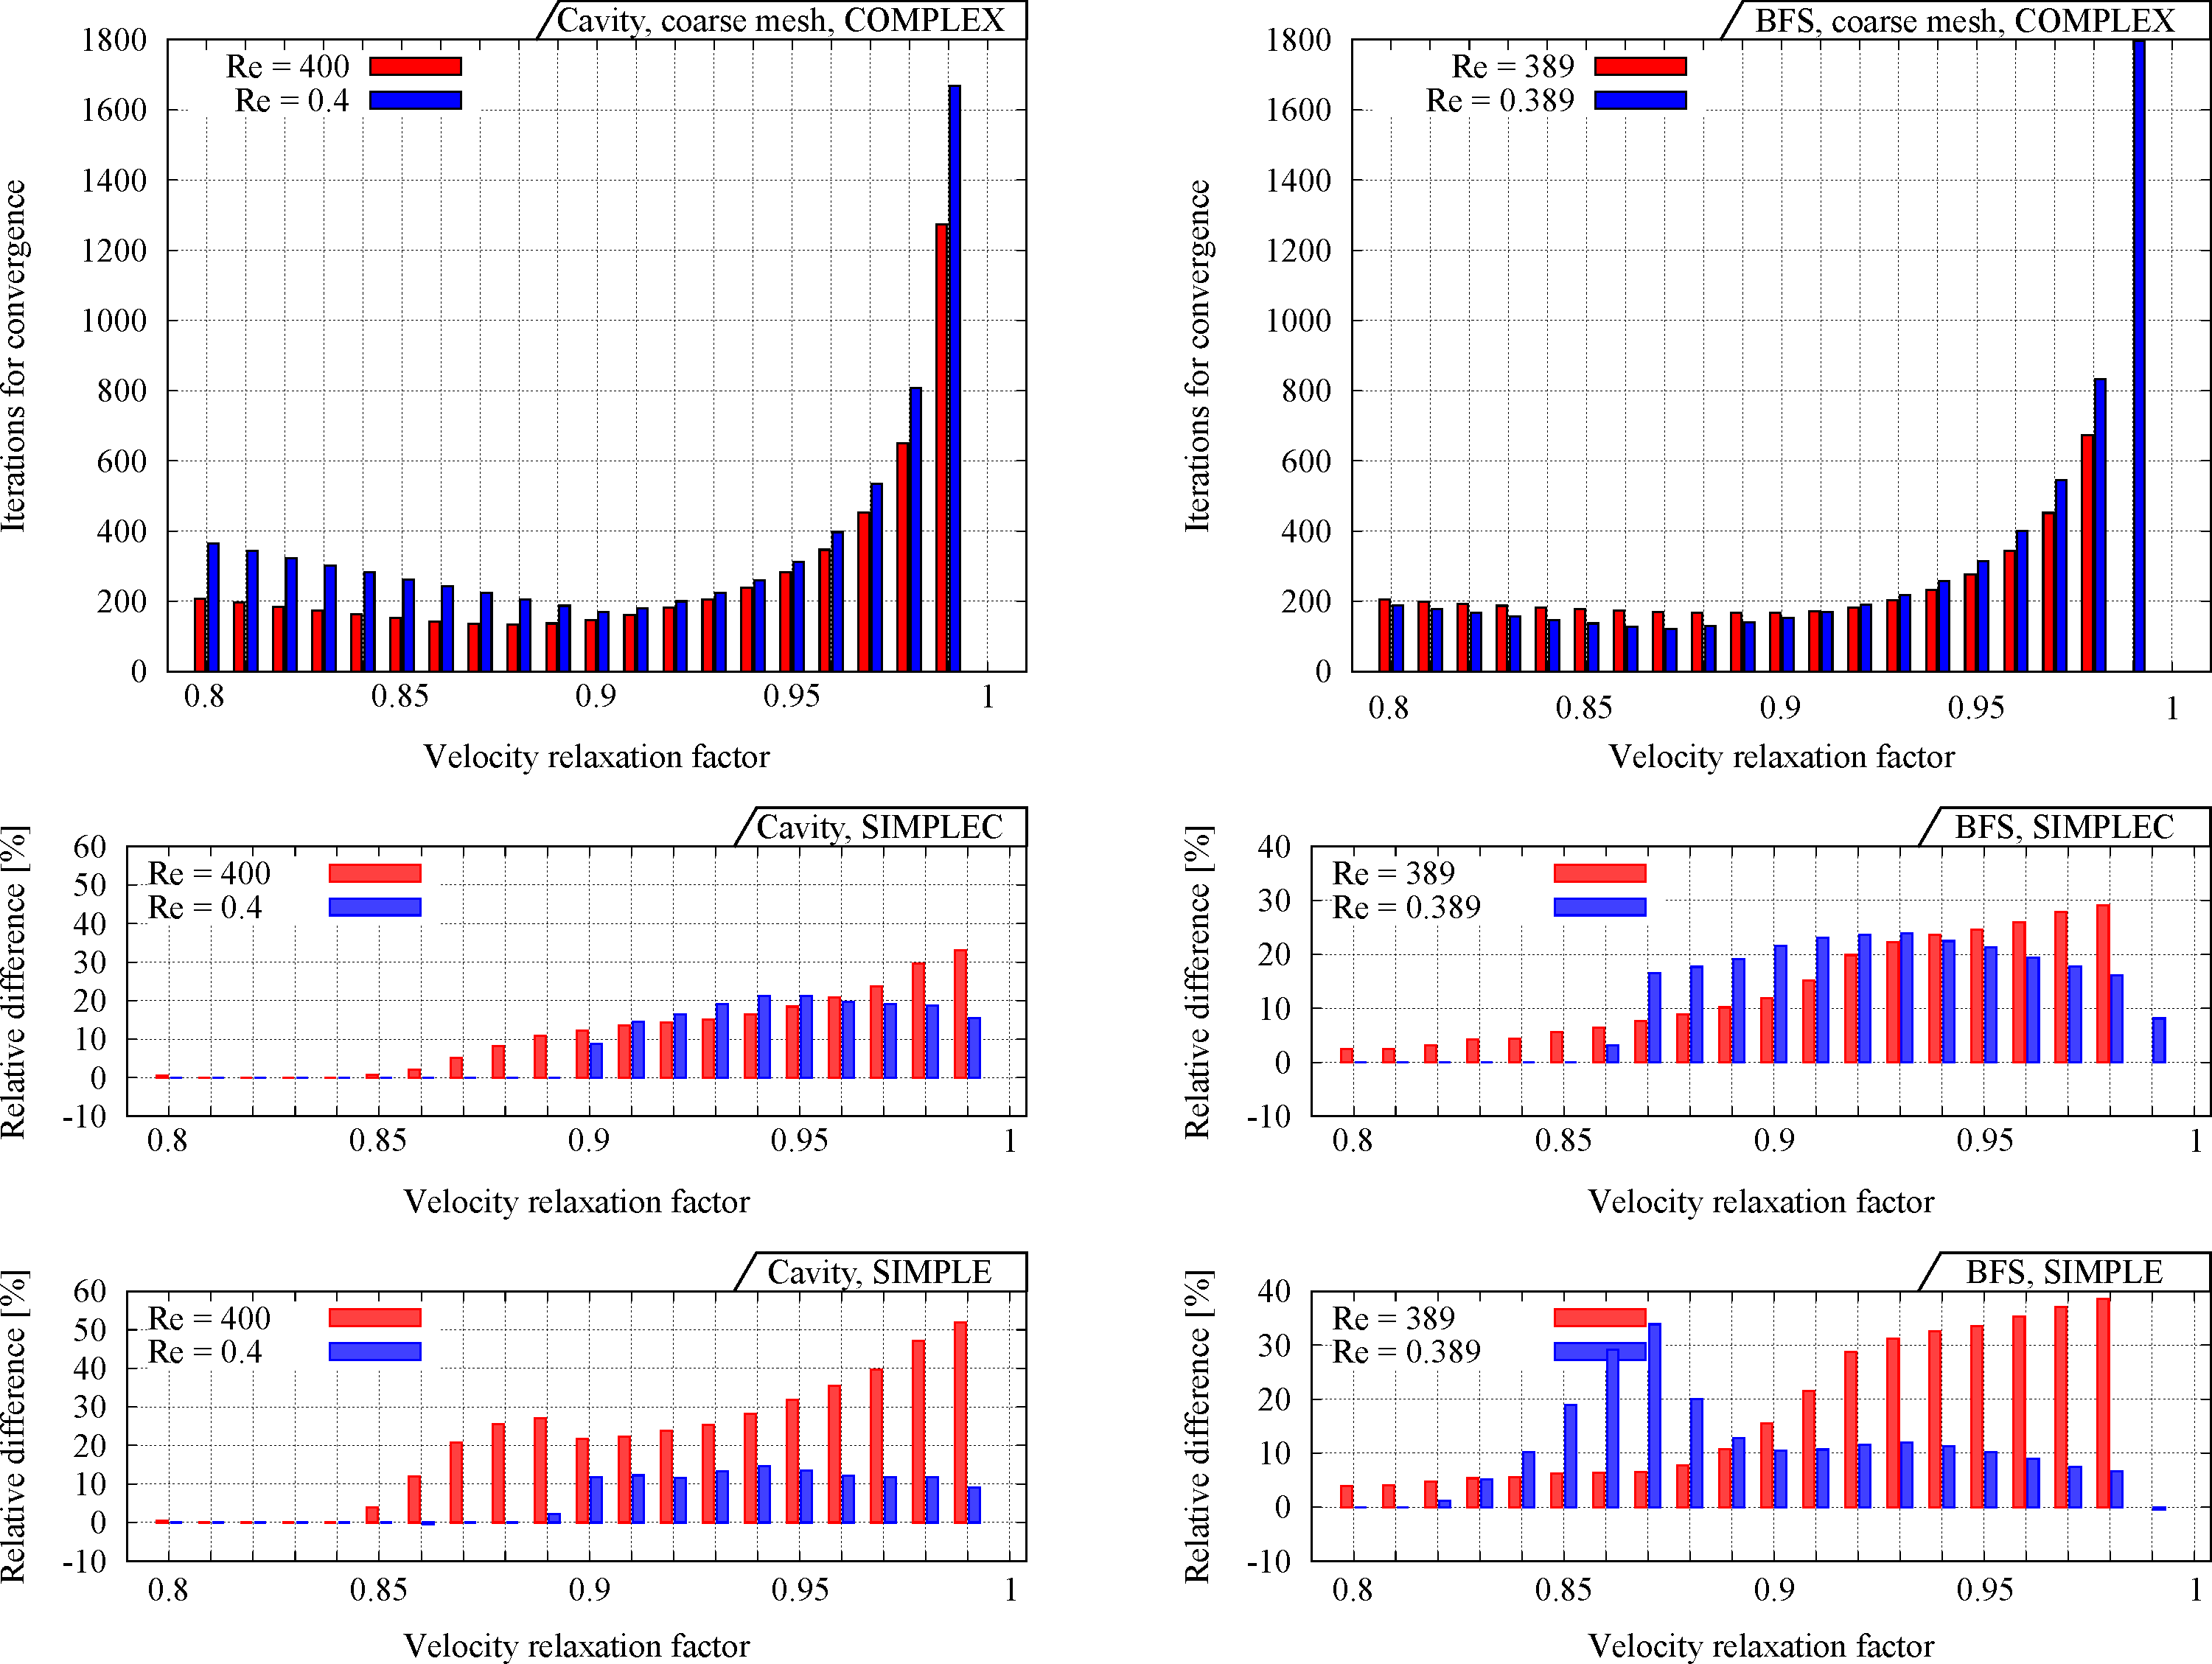
\includegraphics[width=17cm]{fig/Results/complexCoarse.pdf}
\caption{Comparison of the number of iterations required for convergence between COMLEX, SIMPLEC and SIMPLE algorithms using the coarse mesh refinement level. On the left are the results of the Cavity case and on the right, those respective to the BFS.}
\label{Fig:complexCoarse}
\end{figure}

\begin{figure}[t!]
\centering
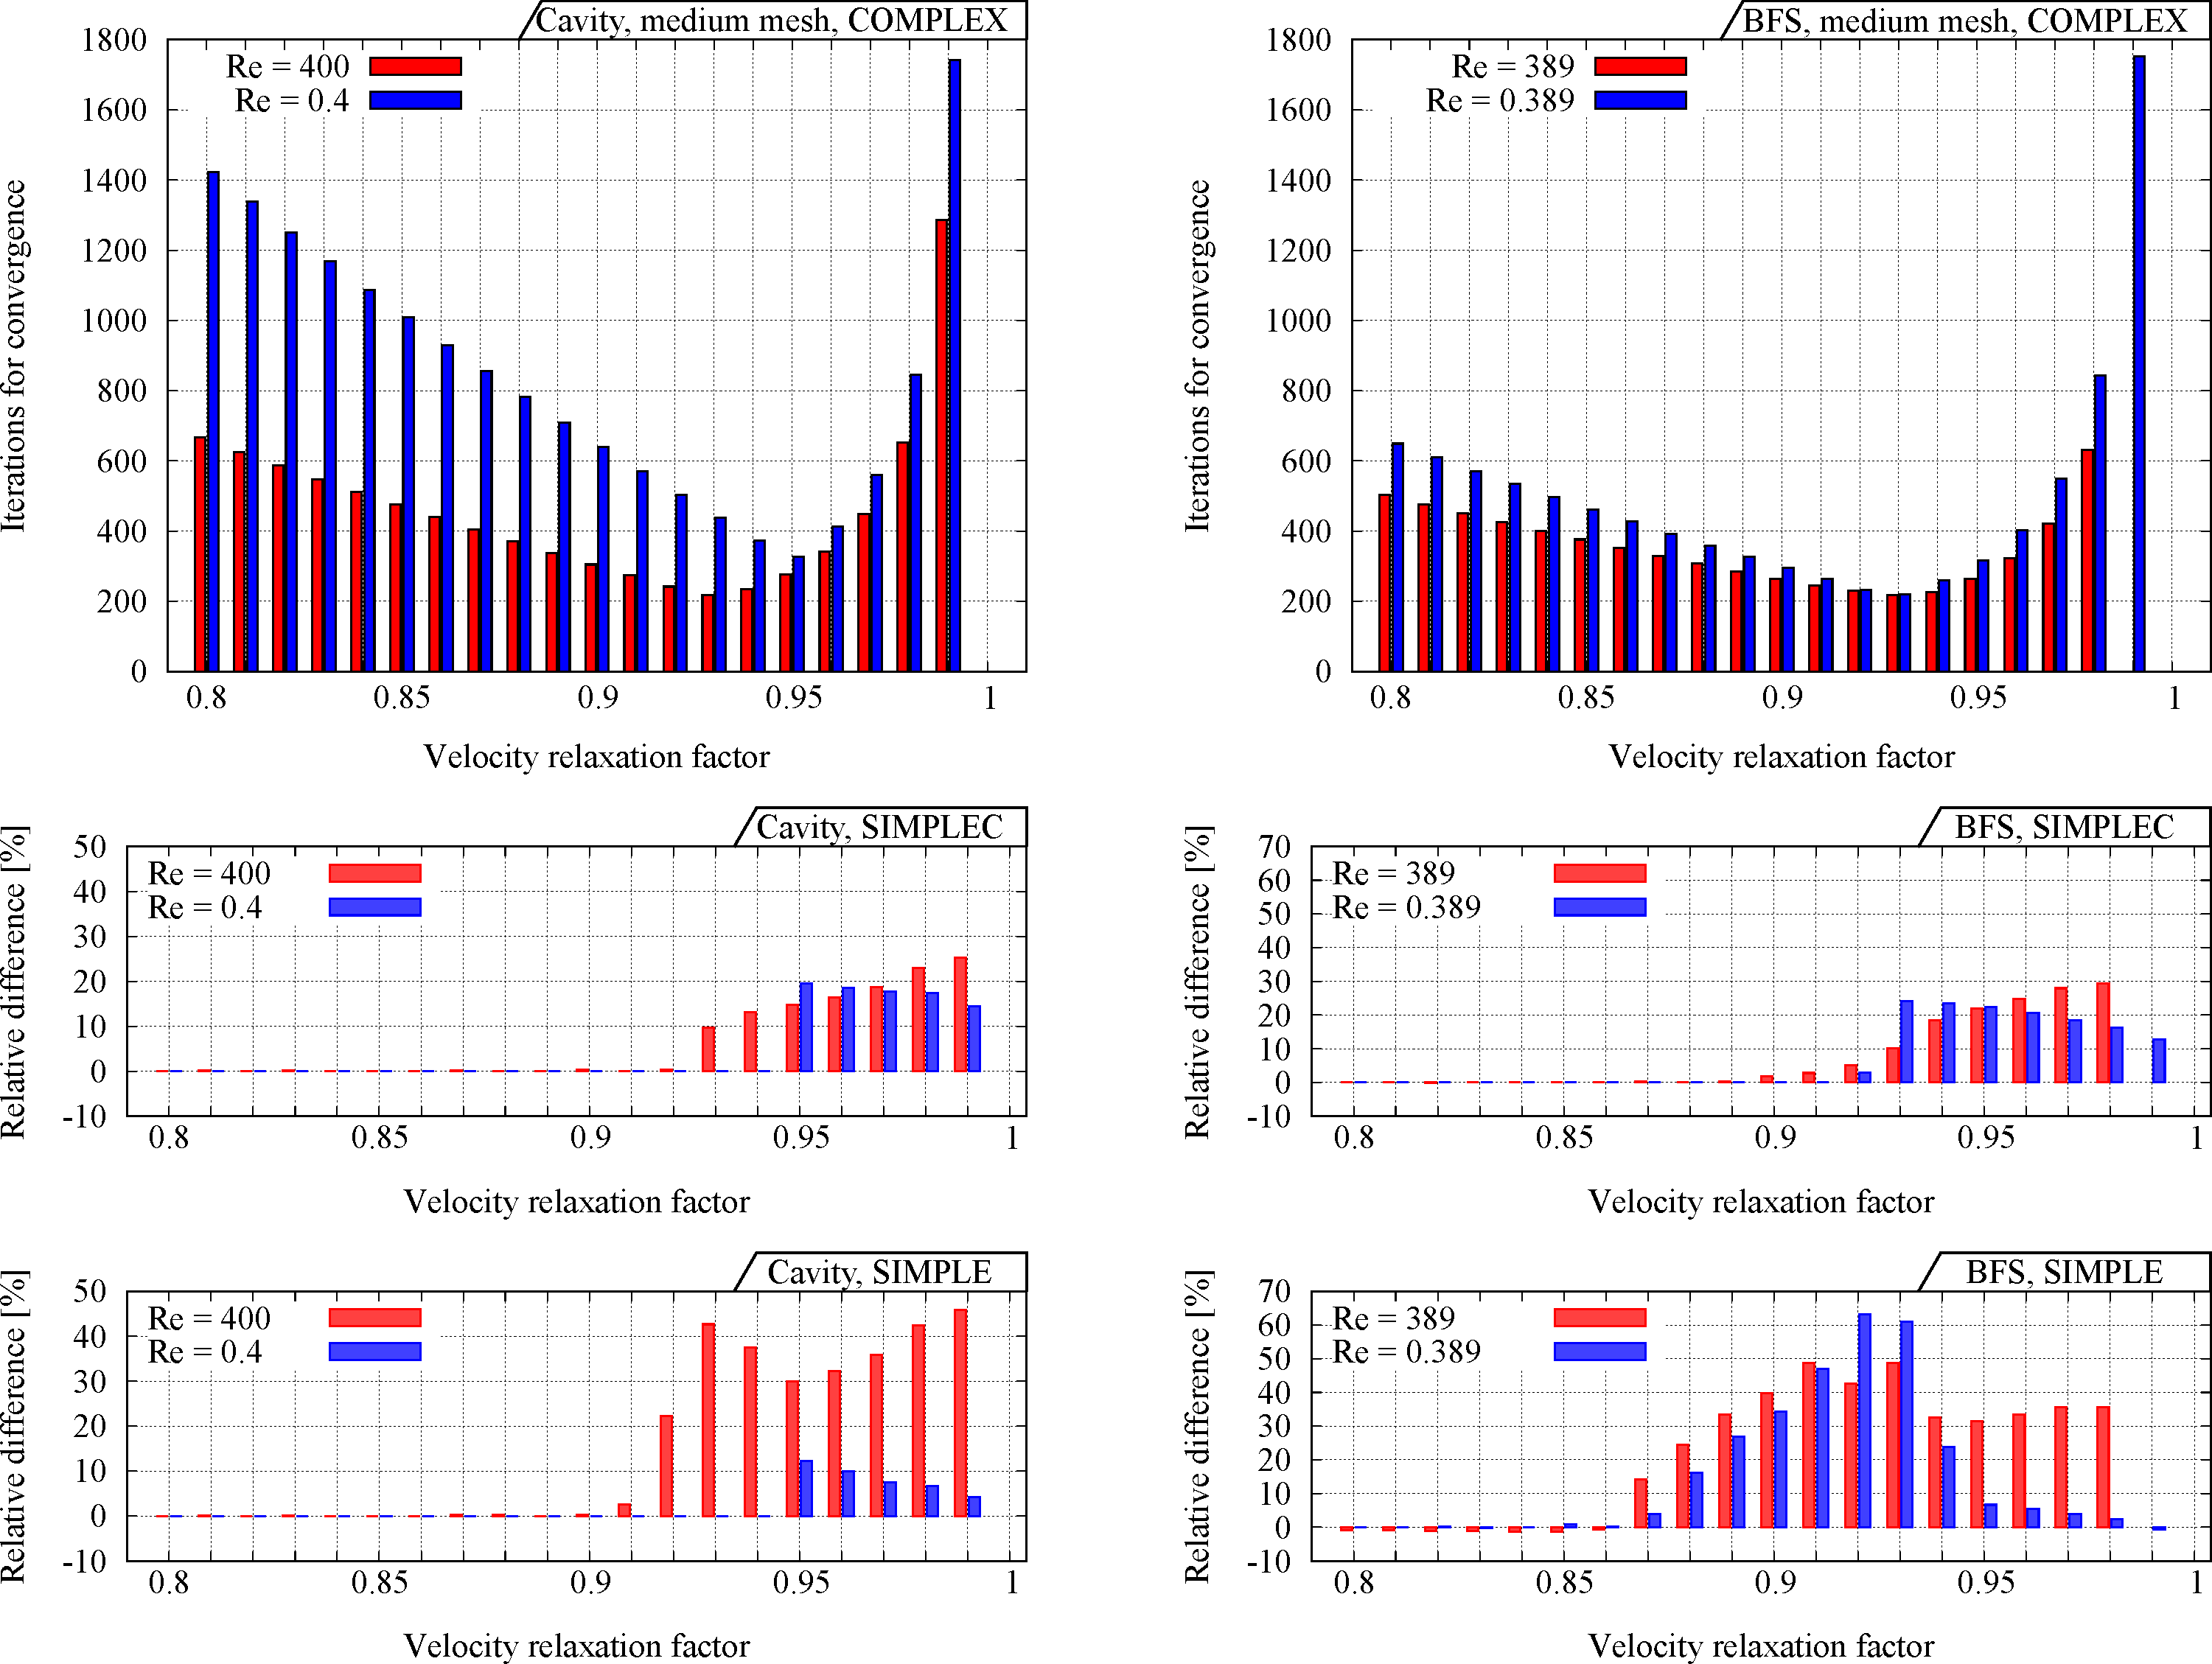
\includegraphics[width=17cm]{fig/Results/complexMedium.pdf}
\caption{Comparison of the number of iterations required for convergence between COMLEX, SIMPLEC and SIMPLE algorithms using the medium mesh refinement level. On the left are the results of the Cavity case and on the right, those respective to the BFS.}
\label{Fig:complexMedium}
\end{figure}

\begin{figure}[t!]
\centering
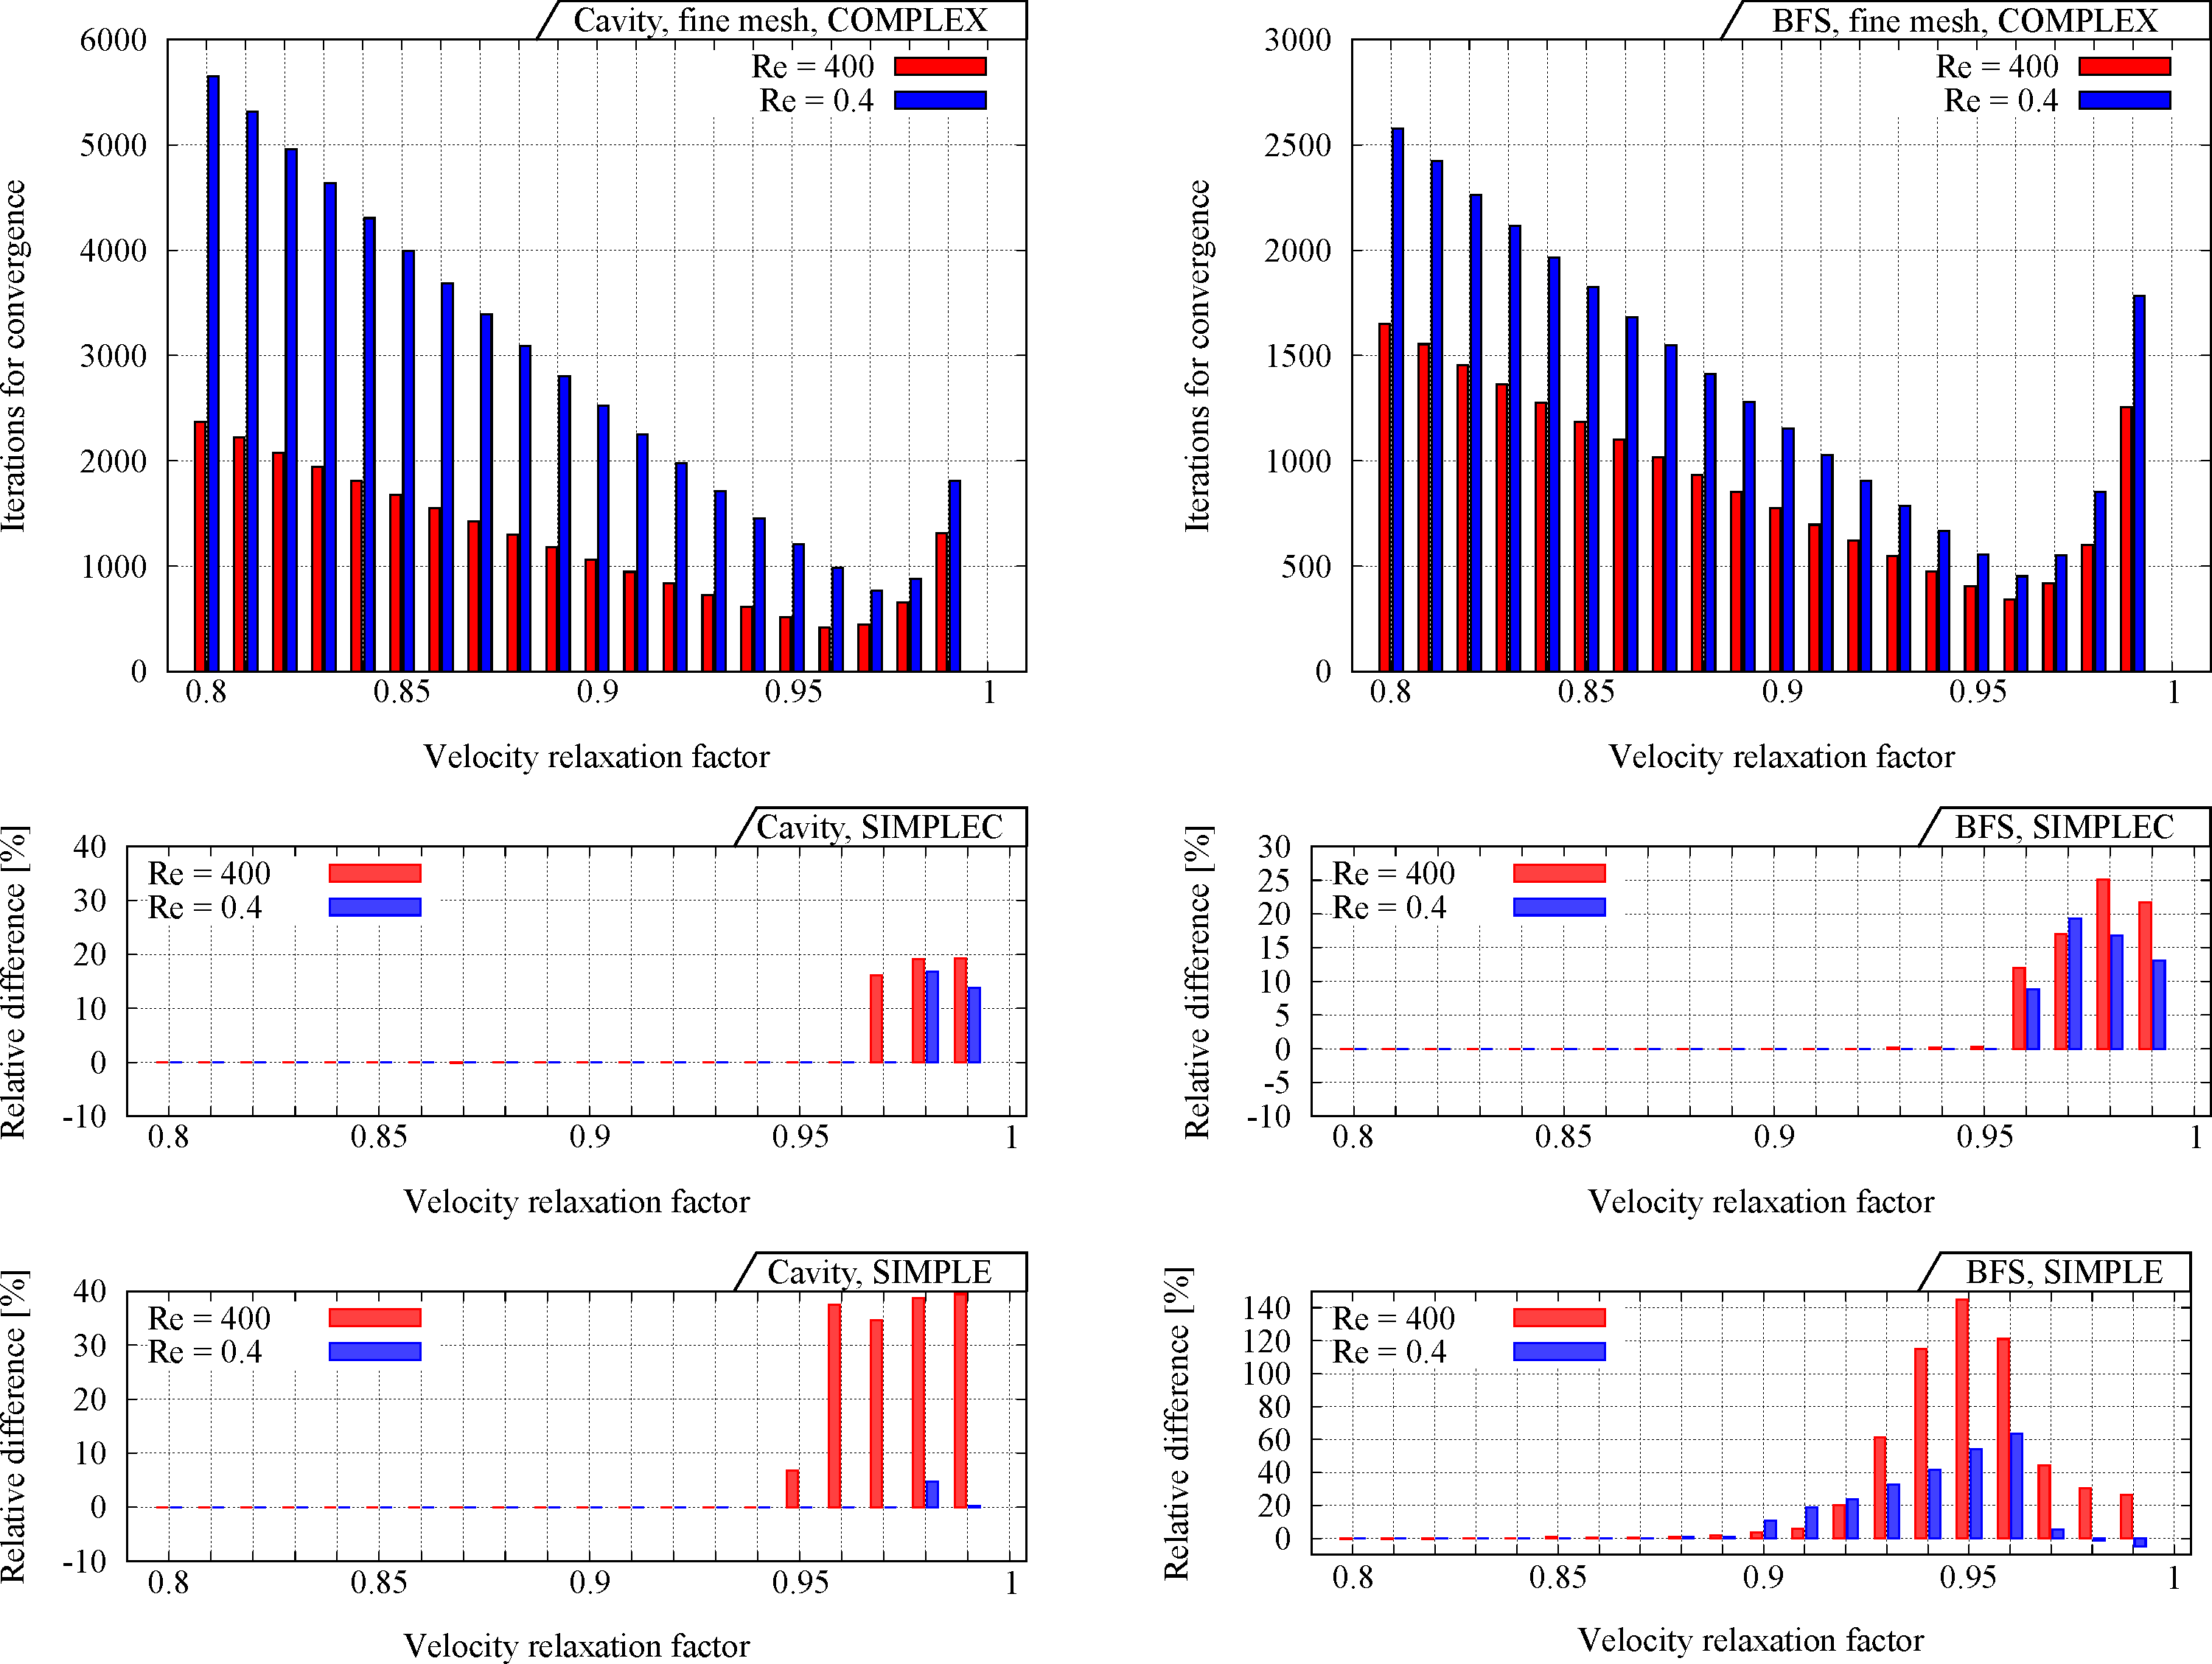
\includegraphics[width=17cm]{fig/Results/complexFine.pdf}
\caption{Comparison of the number of iterations required for convergence between COMLEX, SIMPLEC and SIMPLE algorithms using the fine mesh refinement level. On the left are the results of the Cavity case and on the right, those respective to the BFS.}
\label{Fig:complexFine}
\end{figure}

The results are presented in the Figs.~\ref{Fig:complexCoarse},~\ref{Fig:complexMedium} and \ref{Fig:complexFine} which are respective to the three refinement mesh levels. Each figure includes six bar plots arranged in three rows and two columns. On the right and left columns, the results of the Cavity and BFS simulations are presented respectively. In the first row, the absolute number of iterations at convergence for the COMPLEX method simulations are indicated. Relative to these simulations, the second and third row display the relative number of iterations in percentage for the SIMPLEC and SIMPLE methods respectively,
\begin{equation}
RI(\omega_u)
=
\dfrac
{NI_S(\omega_u) - NI_C(\omega_u)}
{NI_C(\omega_u)}
\times
100\%,
\end{equation}
where $NI_S(\omega_u)$ is the absolute number of iterations required at convergence for the SIMPLEC or SIMPLE method as appropriate when using a relaxation factor of momentum equal to $\omega_u$ and $NI(\omega_u)_C$. 
 In all plots, the blue bars are respective to the relative low Reynolds simulations while the red ones are respective to the relative high Reynolds ones.   

In general, the difference between COMPLEX and the other studied methods is relevant for high values of the momentum relaxation factor $\omega_u$. Examining the absolute number of iterations of COMPLEX, the  value of $\omega_u$ in which the complex method has the best convergence is coincident with the start point from which the differences between the methods become significant. This last observation may be interpreted as COMPLEX has a lower minimum of the required iterations in order to converge and that the decay of the convergence caused by an excessive value of $\omega_u$ is better handled by the COMPLEX method. An hypothesis for the previous reaction of the methods may be explained by considering that a higher relaxation factor of the momentum equation leads to a higher divergence of the velocity field, since this constraint is naturally not imposed in the momentum balance. With this in mind, the COMPLEX strategy includes a numerical correction for this deviation which helps to an enhanced prediction of the pressure in these conditions.

The results are sensitive to the mesh refinement level. Analysing the absolute number of iterations of the COMPLEX method, it is observed that the reduction of the number of iterations when increasing the momentum relaxation factor raises up with mesh refinement. This also deviates the minimum iterations point to the right direction in concordance with a higher value of $\omega_u$. 

The mesh refinement level affects the relative differences between the methods. The range of $\omega_u$ in which COMPLEX converges better is wider in the coarse mesh than in the fine mesh. Namely, this range start from $\omega_u = 0.85$ in the coarse mesh and from $\omega_u = 0.95$ in the fine one.

In regard to the Reynolds number influence on COMPLEX it may be assert that for the relative high Reynolds number, a less iterations are required to reach the convergence criteria. This property of COMPLEX is also observed when comparing it with SIMPLE and SIMPLEC. Here, the iteration reduction required for convergence is higher for the relative high Reynold problems. A similar effect is also noted in the range in which COMPLEX is more convergent. As pointed out before, the range of advantage of COMPLEX regarding the $\omega_u$ value starts at the point where the iteration number is approaching a minimum. This trend is also observed in the high Reynolds simulations since the wider range of advantage of COMPLEX compared with the low Reynolds problems may be justified since the minimum iterations number occurs with a lower value of $\omega_u$.

To conclude this analysis, it is remarked that in almost all cases (Cavity or BFS, mesh refinement level $\omega_u$ value, and Reynolds number) the COMPLEX method is superior in terms of convergence than both, the SIMPLE and SIMPLEC method.

\section{Conclusions}
\label{sec:conclusions}
This paper presented an new strategy to couple velocity and pressure in the context of the FVM which is called as the COMPLEX method. This proposal is based on the SIMPLEC algorithm where the neighbour velocity approximation is enhanced using a Taylor expansion. The resulting expression requires the definition of a velocity gradient which is proposed to be a scalar matrix where its value is computed solving the mass balance equation. The differences between COMPLEX and SIMPLEC may be grouped in a term, named complex term, which is relaxed in order to study its influence on the convergence of the numerical method. 

The COMPLEX method is formally analysed using a Fourier decomposition of the error. In particular, it is compared with the SIMPLEC method in a framework of a one-dimensional Navier-Stokes problem. In view of the study, the COMPLEX method is more stable than SIMPLEC when employing high relaxation values of the momentum equation. On the other hand, for relative low values of the relaxation factor, both methods, COMPLEX and SIMPLEC are equivalent in regards to the convergence rate.

The COMPLEX formulation was studied with two three dimensional problems, the cubic cavity and the BFS cases. For each test, two different Reynodls conditions were analysed. In a first instance, the optimal value of the complex factor $\kappa$  was investigated. An exhaustive study of more than 1500 simulations was performed where the total number of iterations to reach a convergence criteria as function of the momentum relaxation factor, the complex factor $\kappa$ and the Reynolds number, was measured. Based on the stability behaviour and convergence rate of the simulations, a complex factor of $\kappa = 0.2$ was chosen as the most suitable value for the method in the conditions proved. After this point, the COMPLEX method was compared with SIMPLE and SIMPLEC. Here, each problem was solved using three different mesh refinements and varying the Reynolds number as the analysis before. The results proved that the COMPLEX method has advantages in terms of the convergence speed. This improvement was recognized in the range of high values of the momentum relaxation factor. This behaviour of COMPLEX was also verified via the Fourier analysis carried out in Section~\ref{sec:fourier}. This range is longer in coarse meshes which increases the advantage of COMPLEX against the other methods. Another finding was that for high Reynolds number the COMPLEX method has a better convergence than cases with relative lower Reynolds number where the relative difference with the SIMPLE algorithm was particularly significant.

The COMPLEX method is a promising numerical strategy in order to speed up the convergence of segregated algorithms. The implementation of this strategy is simple since it is performed by adding a unique term on the pressure equation in the SIMPLEC formulation.  The main advantage of the current method is that its performance is equal or better than SIMPLEC or SIMPLE. COMPLEX is an advisable method when the prediction of the velocity gets away from the divergence free condition as it is the case of high relaxation factors or high Reynolds numbers.

A challenge of future work is the improvement of the approximation defined in Eq.~(\ref{Eq:scalarMatrix}) (scalar matrix assumption of the velocity gradient). This hypothesis has no error in one-dimensional problems where COMPLEX was proved to be significantly better than SIMPLEC on the basis of the Fourier analysis.


\bibliographystyle{plain}
\bibliography{main}

\end{document}
